\RequirePackage[l2tabu,orthodox]{nag}

% TODO: decide if one-sided/two-sided
%\documentclass[headsepline,footsepline,footinclude=false,fontsize=11pt,paper=a4,listof=totoc,bibliography=totoc,BCOR=12mm,DIV=12]{scrbook} % two-sided
\documentclass[headsepline,footsepline,footinclude=false,oneside,fontsize=11pt,paper=a4,listof=totoc,bibliography=totoc]{scrbook} % one-sided

\input{settings/packages}
\input{settings/settings}
% Basic information for cover & title page
\newcommand*{\getUniversity}{Technische Universität München}
\newcommand*{\getFaculty}{Department of Informatics}
\newcommand*{\getTitle}{A Job Scheduling Algorithm for Malleable Jobs in Invasive Resource Management Systems}
\newcommand*{\getTitleGer}{Ein Job Scheduling Algorithm für Formbar Jobs in Invasive Ressource Management Systeme}
\newcommand*{\getAuthor}{Nishanth Nagendra}
\newcommand*{\getDoctype}{Master's Thesis in Informatics}
\newcommand*{\getSupervisor}{Prof. Dr. Michael Gerndt}
\newcommand*{\getAdvisor}{M.Sc. Isaias Alberto Compres Urena}
\newcommand*{\getSubmissionDate}{May 15, 2015}
\newcommand*{\getSubmissionLocation}{Munich}

% TODO: add custom commands etc.


% TODO: remove if glossary not needed
\input{glossary/terms}
\input{glossary/acronyms}

\begin{document}

\input{pages/cover}

\frontmatter{}

\input{pages/title}
\input{pages/disclaimer}
\addcontentsline{toc}{chapter}{Acknowledgments}
\thispagestyle{empty}

\vspace*{2cm}

\begin{center}
{\usekomafont{section} Acknowledgments}
\end{center}

\vspace{1cm}
\noindent
%TODO: Acknowledgments
I would like to sincerely thank \textit{Isa\'{i}as A. Compr\'{e}s Ure\~{n}a} for his constant support and guidance throughout the thesis through our long and fruitful discussions. He has been extremely patient and generous in providing his time for discussions on topics that were challenging for me but necessary to understand for working in this research direction. The constructive discussions along with his advice have been really valuable to me as a student.\\ \\
%%%%%%%%%%%%%%
I am extremely grateful to \textit{Prof. Dr. Michael Gerndt} for providing me with this wonderful opportunity to be involved in such an interesting project and to work very closely with his research group. He has been very supportive throughout the length of the time i have been involved as a student working in the Chair for Architecture of Parallel and Distributed Systems. Despite his busy schedule, I have had the opportunity for numerous discussions with him that have helped me to gain critical advice for my thesis and other related tasks.
\cleardoublepage{}

\chapter{\abstractname}
Invasive Computing is a novel paradigm for the design and resource-aware programming of future parallel computing systems. It enables the programmer to write resource aware programs and the goal is to optimize the program for the available resources. Traditionally, parallel applications implemented using MPI are submitted with a fixed number of MPI processes to execute on a HPC (High Performance Computing) system. This results in a fixed allocation of resources for the job. Modern techniques in scientific computing such as AMR (Adaptive Mesh Refinement) result in applications exhibiting complex behaviors where their resource requirements change during execution. Invasive MPI is an ongoing research effort to provide MPI extensions for the development of Invasive MPI applications that will result in jobs which are resource-aware for the HPC systems and can utilize such AMR techniques. Unfortunately, using only static allocations result in these applications being forced to execute using their maximum resource requirements that may lead to inefficient resource utilization. In order to support such kind of parallel applications at HPC centers, there is an urgent need to investigate and implement extensions to existing resource management systems or develop a new system. This thesis has extended the previous work during which a protocol was developed for the intgeration of invasive resource management into existing batch systems. In this work, we have explored the idea of separating the concerns of batch and runtime scheduling into two different software layers / components in contrasts to existing systems where both are merged together. Specifically, This thesis has investigated and implemented a job scheduling algorithm in accordance with the new protocol developed earlier for supporting such an invasive resource management. An early prototype that can simulate the negotiation between batch and runtime scheduler using their respective scheduling algorithms for a HPC workload comprising different job types has been accomplished.\par

%TODO: Abstract



\microtypesetup{protrusion=false}
\tableofcontents{}
\microtypesetup{protrusion=true}
\listoffigures{}
\listoftables{}

\mainmatter{}

\chapter{Introduction}\label{chapter:introduction}
Over the last two decades, the landscape of Computer Architecture has changed radically from Sequential to Parallel . Due to the limiting factors of technology we have moved from single core processors to multi core processors having a network interconnecting them. Traditionally, The approach of designing algorithms has been sequential, but designing algorithms in parallel is gaining more importance now to better utilize the computing power available at our disposal. Another important trend that has changed the face of computing is an enormous increase in the capabilities of the networks that connect computers with regards to speed, reliability etc. These trends make it feasible to develop applications that use physically distributed resources as if they were part of the same computer. A typical application of this sort may utilize processors on multiple remote computers, access a selection of remote databases, perform rendering on one or more graphics computers, and provide real-time output and control on a workstation. Computing on networked computers("Distributed Computing") is not just a subfield of parallel computing as the basic task of developing programs that can run on many computers at once is a parallel computing problem. In this respect, the previously distinct worlds of parallel and distributed computing are converging.\\ \par
\noindent
As technology advances, we have newer problems or applications that demand larger computing capabilities which push the limits of technology giving rise to newer advancements. The performance of a computer depends directly on the time required to perform a basic operation and the number of these basic operations that can be performed concurrently. A metric used to quantify the performance of a computer is FLOPS(floating point operations per second). The time to perform a basic operation is ultimately limited by the "clock cycle" of the processor, that is, the time required to perform the most primitive operation. The term \textbf{\textit{High Performance Computing(HPC)}} refers to the practice of aggregating computing power(multiple nodes with processing units interconnected by a network in a certain toplogy) or the use of parallel processing for running advanced application programs efficiently, reliably and quickly. The term applies especially to systems that function above a \textbf{\textit{teraflop}} or \textbf{\textit{$10^{12}$}} floating-point operations per second. The term HPC is occasionally used as a synonym for Supercomputer that work at more than a \textbf{\textit{petaflop}} or \textbf{\textit{$10^{15}$}} floating-point operations per second. The most common users of HPC systems are scientific researchers, engineers, government agencies including the military, and academic institutions. In general, HPC systems can refer to Clusters, Supercomputers, Grid Computing etc. and they are usually used for running complex applications.\\ \par
\noindent
A \textbf{\textit{Batch System}} is used to manage the resources in a HPC System. It is a middleware that comprises of two major components namely the \textbf{\textit{Resource Manager}} and \textbf{\textit{Scheduler}}. The role of a Resource Manager is to act like a glue for a parallel computer to execute parallel jobs. It should make a parallel computer as easy to use as a PC. A programming model such as \textbf{\textit{Message Passing Interface(MPI)}} for programming on distributed memory systems would typically be used to manage communications within a parallel program by using the MPI library functions. A Resource Manager allocates resources within a HPC system, launches and otherwise manages Jobs. Some of the examples of widely used open source as well as commercial resource managers are \textbf{\textit{SLURM, TORQUE, OMEGA, IBM Platform LSF}} etc. Together with a scheduler it is termed as a Batch System. The role of a job scheduler is to manage queue(s) of work when there is more work than resources. It supports complex scheduling algorithms which are optimized for network topology, energy efficiency, fair share scheduling, advanced reservations, preemption, gang scheduling(time-slicing jobs) etc. It also supports resource limits(by queue, user, group, etc.). Many batch systems provide both resource management and job scheduling within a single product (e.g. LSF) while others use distinct products(e.g. Torque Resource Manager and Moab Job Scheduler). Some other examples of Job Scheduling Systems are \textbf{\textit{LoadLeveler, OAR, Maui, SLURM etc.}}\\ \par
\noindent
Existing Batch Systems usually support only static allocation of resources to Jobs/Applications before they start which means the resources once allocated are fixed for the lifetime of the application. The complexity of applications have been growing especially when we consider advanced techniques in Scientific Computing like \textbf{\textit{Adaptive Mesh Refinement(AMR)}} where applications exhibit complex behavior by changing their resource requirements during execution. The Batch Systems of today are not equipped to deal with such kind of complex applications in an intelligent manner apart from giving the Job the maximum number of resources before it starts that will result in sheer wastage of resources leading to poor resource utilisation. In order to support such parallel adaptive applications at HPC centers there is an urgent need to investigate and implement extensions to existing resource management systems or develop an entirely new one. These supporting infrastructures must be able to handle the new kind of adaptive applications and the legacy static jobs intelligently keeping in mind that they should now be able to achieve much higher system utilisation, energy efficiency etc. compared to their predecessors due to the elasticity of the applications.

\section{Invasive Computing}
The throughput of HPC Systems depends not only on efficient job scheduling but also on the type of jobs forming the workload. As defined by Feitelson, and Rudolph, Jobs can be classified into four categories based on their flexibility:
\begin{itemize}
\item \textbf{\textit{Rigid Job:}} Requires a fixed number of resources throughout its execution.
\item \textbf{\textit{Moldable Job: }} The resource requirement of the job can be molded or modified by the Batch System before starting the job(e.g. to effectively fit alongside other rigid jobs). Once started its resource set cannot be changed anymore.
\item \textbf{\textit{Evolving Job: }} These kind of jobs request for resource expansion or shrinkage during their execution. Applications that use Multi-Scale Analysis or Adaptive Mesh Refinement(AMR) exhibit this kind of behavior typically due to unexpected increases in computations or having reached hardware limits(e.g. memory) on a node.
\item \textbf{\textit{Malleable Job: }} The expansion and shrinkage of resources are initiated by the batch system in contrast to the evolving jobs. The application adapts itself to the changing resource set.
\end{itemize}
The first two types fall into the category of what is called as the static allocation since the allocation of rigid and moldable jobs must be finalized before the job starts. Whereas, the last two types fall under the category of dynamic allocation since this property of expanding or shrinking evolving and malleable jobs(together termed adaptive jobs) happens at runtime. Adaptive Jobs hold a strong potential to obtain high system performance. Batch systems can substantially improve the system utilization, throughput and response times with efficient shrink/expand strategies. Similarly, applications also profit when expanded with additional resources as this can increase application speedup and improve load balance across the job\textquotesingle s resource set.\\ \par
\noindent
Invasive Computing is a novel paradigm for the design and resource-aware programming of future parallel computing systems. It enables the programmer to write efficient resource aware programs. This approach can be used to allocate, execute on and free resources during execution of the program. This results in adaptive applications at runtime that can expand and shrink in the number of their resources. This will also potentially help to achieve much better resource utilisation and energy efficiency if efficient shrink/expand strategies can be used for all the jobs/applications. HPC infrastructure like Clusters, Supercomputers execute a vast variety of jobs, majority of which are parallel applications. These centers use intelligent resource management systems that should not only perform tasks of job management, resource management and scheduling but also satisfy important metrics like higher system utilization, job throughput and responsiveness. Traditionally, MPI applications are executed with a fixed number of MPI processes but with Invasive MPI they can evolve dynamically at runtime in the number of their MPI processes. This in turn supports advanced techniques like AMR where the working set size of applications change at runtime. These advancements result in adaptive applications at runtime and therefore need an intelligent resource management system that can provide efficient resource utilization at HPC centers. They should also now be able to achieve much higher system utilisation, energy efficiency etc. compared to their predecessors due to elasticity/adaptivity of the applications.\par
\noindent
\\Under the collaborative research project funded by the \textbf{German Research Foundation(DFG)} in the \textbf{Transregional Collaborative Research Centre 89(TRR89)}, research efforts are being made to investigate Invasive Computing approach vertically at different levels of abstraction right from the hardware up to the programming model and including the applications. \textbf{Invasive MPI} is an effort towards invasive programming with MPI where the application programmer has MPI extensions available for specifying at certain safe points in the program to allow for elasticity which means that the application can evolve.\\ \par

\section{Dynamic Resource Management}
Two of the most widely used resource managers on HPC systems are \textbf{SLURM} and \textbf{TORQUE}. The two major components in general of any sophisticated resource manager are the batch scheduler and the process manager. The Process Manager is responsible for launching the jobs on the allocated resources and managing them throughout their lifetime. Examples of process manager are \textbf{\textit{Hydra, SLURM Daemon(slurmd)}} etc. The Process Managers interact with the processes of a parallel application via the \textbf{Process Management Interface(PMI)}. In order to support Invasive Resource Management, The following components will be implemented: \textbf{\textit{iScheduler}}(Batch Scheduler for Invasic Jobs) built as an extension into an existing batch system and \textbf{\textit{iDRScheduler}}(Invasive Distributed Run TIme Scheduler) similar to a controller daemon which will sit between the batch scheduler and the process manager. \textbf{SLURM} is the choice of an existing batch system on which this prototype will be implemented for demonstrating Invasive Computing and below is a high level illustration of the architecture for such an Invasive Resource Management.\\ \par
\begin{figure}[!htbp]
\centering
\includegraphics[width=0.8\textwidth, height=60mm]{./figures/architecture.pdf}
\caption{Invasive Resource Management Architecture}
\label{fig:1}
\end{figure}
\noindent
The figure\ref{fig:1} illustrates the proposed Invasive Resource Management Architecture. In addition to a Job Queue for Legacy static jobs, we now have an additional Job Queue for Invasic(Adaptive) Jobs. The existing Batch Scheduler needs to be extended in order to schedule these new type of Invasic Jobs and a new component called \textbf{\textit{Invasic Scheduler(iScheduler)}} is responsible for this. In contrast to modifying an existing system to support Invasive Resource Management, A new component called \textbf{\textit{Invasive Distributed Run Time Scheduler(iDRScheduler)}} is proposed which sits between the Batch Scheduler and Process Manager. The objective of such a multi-level approach is to avoid modifying the existing system which will be a substantially large effort and rather have an independent component that caters specifically to Invasic Jobs. It is responsible for managing the resources present in the Invasic paritition used specifically for running Invasic Jobs. With this approach, the existing Legacy Jobs can be served via the existing batch scheduler and the new Invasic Jobs can be served by via iScheduler and iDRScheduler. iDRScheduler talks to the iScheduler via a protocol called the Negotiation protocol to receive Invasic Jobs dispatched from iScheduler which it then launches for execution by performing some run time scheduling like pinning of jobs, expand/shrink etc.\\ \par
\noindent
The new components proposed in the architecture help achieve the objective of supporting dynamic resource management for invasic applications. iScheduler is responsible for scheduling Invasic Jobs. The scheduling decisions are communicated via negotiation protocol to iDRScheduler and these decisions are basically job(s) selected via a scheduling algorithm to be submitted for execution. The decisions will be made on the basis of Resource Offers sent by iDRScheduler which creates these resource offers based on the state of the partition. Upon receiving a resource offer, iScheduler will either accept it by selecting jobs from the queue that can be mapped to this offer or reject it. A Resource Offer can represent real or virtual resources because the iDRScheduler can also present a virtual view of resources in the hope of getting a mapping of jobs to offer that is more suitable to satisfy its local metrics such as resource utilization, power stability, energy efficiency etc. It can either accept or reject the mapping received from iScheduler. Similar to iDRScheduler, the iScheduler makes its decisions to optimize for certain local metrics such as high job throughput, reduced job waiting times, deadlines, priorities etc. This highlights the mismatching policies/metrics for which both the iDRScheduler and iScheduler make their decisions on and hence both will be involved in some kind of a negotiation via the protocol to reach a common agreement. iDRScheduler is an independent entity introduced with the purpose of inter-operating with existing batch systems rather than replacing them with an entirely new one. It may be possible that in the future this component will not be a separate entitiy but will be built into the batch system itself.\\ \par
\noindent
\textbf{\textit{Shrink/Expand Strategies: }}There are several strategies one may employ to tackle adaptive applications during runtime and take decisions that can lead to higher system utilisation, energy efficiency etc.:
\begin{itemize} 
\item Let us consider that at any given point of time there are some Invasic Jobs running in the system. If the parallel runtime environment is able to anticipate that in the near future, there may be a large window of free resources available because some applications may shrink according to a prediction of their scalability behavior with the help of run time profiling and collected performance data then iDRScheduler can provide a resource offer to iScheduler. This offer can specify a virtual list of nodes more than what is available in order to get a mapping of jobs. These jobs can then be shrunk and fit into the existing space of resources with the knowledge that they may be able to expand later.
\item Another scenario is where there is an anticipation of a smaller window of resources in the future because some of the currently running applications may expand. In such a case iDRScheduler will provide a resource offer to iScheduler with a virtual list of nodes smaller than what is currently available in order to get a mapping of jobs. These jobs can be then be expanded and fit into the existing space of resources with the knowledge that they may have to shrink later.
\item The third variation could be the case where the runtime anticipates the state of resources to remain the same as the current state for the near future since none of the running applications may expand or shrink. In such a scenario iDRScheduler will send a resource offer that is a list of nodes which is exactly the same as the available resources to iScheduler in order to get a mapping of jobs. These jobs can then be fit into the space of resources available as it is without expanding/shrinking them. 
\end{itemize}
\section{Master Thesis}
The focus of this Master Thesis is to extend the early prototype developed as a part of the guided research in the last few months. It will now give concrete meanings to the negotiation protocol, defining the format of the invasic job records, its constraints, definition of resource offers, feedback reports and most important of all to investigate and develop an efficient job scheduling algorithm at the iScheduler level. Following this closely from the Guided Research would be to continue having an automated testing in place that will help in simulating a workload of jobs, testing the job scheduling algorithm for its correctness, evaluating and analysing the performance of such a prototype for various metrics. Given below is a tentative plan of the activities proposed monthwise starting from November $15$ till May $15$ to be carried out for the duration of 6 months in this Master Thesis.\par
\subsection{Tentative Plan}
\begin{itemize}
\item Literature survey for current/recent related work on batch job scheduling from research groups focusing on problems in the areas of batch scheduling, resource management, middleware etc. In addition to this, defining resource offers, invasic job records and job constraints that can come from a pre-computed performance model of an application during its runtime or could be user defined. Once these tasks have been completed, it will follow up with extending the early prototype by the implementation of these ideas and testing them for correctness using the automated testing feature.
\item Integration of the fake iHypervisor with the real iHypervisor by making it as its plugin. Test this integration for all the earlier development using the automated testing feature for correctness. Review, analyse, fix any errors and repeate the process till the integration is stable. Follow this up by understanding the SLURM's existing scheduling algorithms including the recent Machine Learning approach for a possible reuse or enhancement. Define the format of feedback reports sent by iHypervisor and how they can be processed on the iScheduler side including its storage mechanism(possibly using SLURM's existing database functionalities). Implement these ideas in the prototype and test it thoroughly.
\item Investigate and experiment with basic scheduling algorithms first to later proceed with complex ones. Design and implement a sophisticated scheduling algorithm for mapping jobs from Invasic job queue to the resource offers sent by iHypervisor. This algorithm must perform its decision making by also using the collected history/feedback data about many statistical measures provided by iHypervisor periodically.
\item Implementation of the Job Scheduling Algorithm continues for realizing all the necessary requirements as proposed earlier till it has been successfully implemented and later followed by a lot of functional testing.
\item Test the full prototype along with the other component iHypervisor(Including its Run Time scheduling and Invasive Resource Management) for simple to complex workloads(emulating a queue of invasic jobs possibly including legacy static jobs). Testing also needs to be done with real Invasic applications developed by the \textit{Chair Of Scientific Computing}. Find issues/errors, review, analyse, correct and repeat the process till it is stable and then collect all the results necessary.
\item Coming up with the draft version of the Master Thesis Report followed by reviews, corrections. This process is repeated till the final version is decided. Also prepare the slides for the Master thesis to present them at a later stage.
\end{itemize}
\noindent
\\The above timeline highlights a tentative plan for the activities to be taken up during the Master Thesis and the $6$ items above correspond to these $6$ months of the Thesis in a chronological order. The steps may overlap or shift depending on the progress but the same overall structure will be followed for the Thesis. It will also include in parallel small amounts of documentation in the report as and when necessary during the $6$ month period and not necessarily everything at the end.\par

\chapter{Related Work}\label{chapter:related work}
The problem of job scheduling for adaptive applications as introduced in the previous chapter is really at the intersection of many different problems. In this section, we will look at the some of the relevant work that has happened in the past with respect to batch job scheduling and also briefly look at a subset of the relevant work that has happened with resource-aware programming models and runtime scheduling.\\ \\
%%%%%%%%%%
Substantial amount of work has been done in exploring efficient resource management and scheduling for HPC systems in the past focusing on rigid and moldable jobs. There has been growing interest in the recent years to explore dynamic resource management and scheduling techniques to address the challenges of future exascale machines and the complex applications that will try to exploit this massive parallelism. The complexity of applications are increasing, ex: Scientific applications utilizing \textbf{\textit{Adapative Mesh Refinement(AMR)}} techniques change their working set size as the mesh is refined/coarsened. Dynamically allocating resources to such applications at runtime or other applications which are potentially scalable has the potential to improve resource utilization, energy efficiency, fault tolerance\cite{vadhiyar} and a host of other metrics\cite{abhishek}\cite{osman}. Wolf.et.al\cite{felix} demonstrated such a dynamic resource management approach for supporting evolving jobs by extending the Torque / Maui Batch System to allow dynamic allocations and a dynamic fairness strategy implemented in the Maui Scheduler to efficiently service static and dynamic allocations. Their results showed reduced turnaround and waiting times for applications, while increasing system utilization and throughput. Wolf.et.al\cite{laxmikant} also proposed an extension to this work to further support malleable type of jobs with the help of a communication protocol between the Batch System and the Charm++ runtime which enables the malleability of applications. In combination with their earlier work, The Scheduler now supported a mix of jobs with different types such as rigid, malleable and evolving by using an intelligent algorithm called DBES (Dependency-based expand shrink). Several other efforts have been made earlier in order to support scheduling such a mix of job types\cite{hungershofer}\cite{jamjoom}\\ \\
%%%%%%%%%%%
In contrast to the research efforts mentioned above that focused on the Charm++, there have been several efforts directed towards MPI\cite{georgiou}\cite{travis}\cite{gladys}\cite{gonzalo}\cite{martin}\cite{gonzalo} some of which explored on how to first provide such an adaptive behavior on MPI applications and some on how to support the same with the help of libraries, resource management systems\cite{klein} etc. In the current collaborative research project earlier efforts were directed towards supporting such adaptive programming paradigms in shared memory programming model such as openMP\cite{andreas} and work was also done in MPI\cite{isaias}. The ongoing efforts in this project is to now continue forward in the direction of MPI but to approach the problem vertically at different levels of abstraction such as the programming model, middleware and runtime tuning of applications.\\ \\
%%%%%%%%%
This thesis will mainly focus on the middleware part of this solution stack to support adaptive applications in future HPC systems. Middlewares provide job scheduling for HPC systems and job scheduling has always remained a very active area of research both for theoretical purposes and for practical systems. The most widely used and proven technique running in most of the HPC systems today is \textbf{\textit{backfilling}}. Backfilling was first developed by lifka\cite{david} for the Argonne National Laboratory's IBM SP system to address the need for a new scheduling system on supercomputers and was named as \textbf{EASY}(Extensible Argonne Scheduling System). Feitelson.et.al\cite{ahuva} proposed an extension to backfilling by providing a reservation for every job that could not be started and allowing lower priority jobs from behind in the queue to start if they would not delay these reservations. This was called as \textbf{\textit{Conservative Backfilling}} whereas the one proposed by lifka was called \textbf{\textit{Aggressive Backfilling}} as it provided a reservation to the job only at the front of the queue. Feitelson.et.al\cite{dror} came up with a new approach to backfilling algorithm where a set of jobs from the job queue are looked at once for making a scheduling decision using dynamic programming instead of traversing the queue one job at a time. The claim was that this resulted in better packing of jobs resulting in higher utilization, reduced mean response time and mean slowdown of all jobs. This scheduler was named as \textbf{\textit{LOS(Lookahead Optimizing Scheduler)}}. Efforts have also been made for having intelligent batch scheduling algorithms towards better IO utilization, energy efficiency and several other metrics\cite{zhou}\cite{desai}\cite{yang}\cite{daniel}\cite{dongxu} \\ \\
%%%%%%%%%%
In addition to the standard batch job scheduling for rigid jobs, efforts have also been made in the direction of supporting moldable jobs. Cirne.et.al\cite{wcirne} proposed \textbf{SA(Supercomputer AppLes - Application level scheduler)} that would select on behalf of the user, the appropriate size for a given job from its available sizes. This decision was made based on the state of the resources, job characteristics etc to minimize turnaround time. Sadayappan.et.al\cite{sabin}\cite{srividya}\cite{sudha} proposed several works for moldable scheduling of parallel jobs by using different policies like fair-share, overbooking, and finally considering job's efficiency also in determining the best partition size for the job. They developed an iterative algorithm in order to make the appropriate choice of values for overbooking and efficiency which is inturn based on the scalability characteristics of the job mix.\\ \\
%%%%%%%%
Several efforts have also been made in the direction of scheduling malleable jobs where frameworks have been developed\cite{wcirne1} in order to handle the runtime scheduling of such type of jobs. These frameworks take into consideration several policies and performance / scalability criteria of running applications into its decision making. Deshmeh\cite{deshmeh} proposed a performance prediction tool called \textbf{ADEPT (Automatic Downey-Based Envelope-Constrained Prediction Tool)} that will predict with high accuracy the performance of the application while requiring only few observations. Sudarshan.et.al\cite{sudarshan}\cite{rajesh} proposed a framework that provided support for dynamically resizing the applications. It provided data redistribution algorithms required while reisizing the applications, performance-sensitive scheduling of such applications with the help of smart policies and strategies.\\ \\
%%%%%%%%
Traditionally, Batch Systems have had both batch and runtime scheduling merged together into a single component. In this work, we explore the idea of separating the two concerns into different components for providing a dynamic and flexible scheduling functionality. Such a multi-level approach has usually been observed in the grid and cloud based infrastructures\cite{kwang}\cite{kurowski}\cite{streit}\cite{streit1}. These infrastructures are distributed geographically and employ a local resource manager and scheduler at each of these locations and all of these locations are coordinating by a single centralized broker / service provider. The broker usually engages in some sort of a negotiation\cite{oliver}\cite{roland}\cite{viktor}\cite{rizos} with the different locations / resource providers / sites for availability of resources in order to make the best possible decision for serving its users.

\chapter{Invasive Computing}
\label{chapter:invasive computing}
Invasive Computing\cite{teich} is a novel paradigm for designing and programming future parallel systems. Decreasing feature sizes are motivating a redesign of multi million transistor system-on-chip architectures. This can lead to a dramatic increase in the rates of temporary and permanent faults as well as feature variations. SoCs with 1000 or more processors on a single chip in the year 2020 are foreseen, hence static and central management concepts to control the execution of all resources are no longer appropriate. Invasive Computing allows a program to be resource-aware by which it can explore and dynamically spread its computations to neighbour processors in a phase called as \textbf{\textit{invade}}, then to execute portions of code of high parallelism degree in parallel based on the available invasible region in a given multi-processor architecture in a phase called as \textbf{\textit{infect}}. Later, once the degree of parallelism should be lower again or if it terminates, the program may enter a \textbf{\textit{retreat}} phase where it can deallocate resources and resume execution again, for example, on a single processor. With the help of such resource awareness, the program has the ability to self-organise itself and be immune to faults, feature variations, be highly scalable, show performance gain and record a higher resource utilization metric.\\ \\
This concept would require not just new programming concepts, languages, compilers and operating systems but a radical change in the architectural design of MPSoCs (\textit{Multi-Processor Systems-On-a-Chip}) so as to efficiently support invasion, infection and retreat operations. Some of the main motivations behind the idea of invasive computing are enumerated below:
\begin{itemize}
\item \textbf{\textit{Programmability}} How to map algorithms and programs to 1000 processors or more and how to benefit from the massive parallelism available by tolerating manufacturing defects, feature variations etc.
\item \textbf{\textit{Adaptivity}} Modern applications have unpredictable resource requirements most of which may not be known at compile-time. In addition to this, when different applications are running on a single chip, resource distribution will have to happen dynamically keeping up a high resource utilization and performance. These factors show the need for some sort of hardware / software reconfigurability of the MPSoC.
\item \textbf{\textit{Scalability}} How to efficiently run algorithms and programs on different number of resources?
\item \textbf{\textit{Physical Constraints}} Heat dissipation will be a major bottleneck. Intelligent methods and architectural support to run algorithms at different speeds to exploit parallelism under power reduction is needed.
\item \textbf{\textit{Reliability and Fault-Tolerance}} Applications must be immune to temporal or permanent faults that may be caused due to manufacturing defects, feature variations, degradation etc. This especially has a higher likelihood to happen in the case of future MPSoCs.
%%%%%%%
\end{itemize}
The paradigm of invasive computing offers a new perspective for programming large scale HPC systems. Current resource management systems manage resources via static partitioning among parallel jobs. This is a very rigid approach considering that an application will then be limited to a fixed amount of parallelism it can utilize. This, however, will not be beneficial especially in the case of future exascale systems where if one needs to derive maximum performance then the maximum number of resources will have to be allocated. The application can benefit from invasive programming during certain phases of its runtime by running at maximum parallelism and in the remaining time it can run at a lower parallelism.\\ \\
%%%%%%%
Another motivation is for a specific classes of applications like multi-grid and adaptive grid. Multi-grid applications work on multiple grid levels ranging from fine to coarse grids. On fine grids, more resources could yield better performance and efficiency, whereas on coarse grids fewer resources would be sufficient. In the case of adaptive grid applications, the grid is dynamically refined according to the current solution and the application may go through different levels of parallelism in different phases.\\ \\
%%%%%%%
Scaling the systems to exaflop level would consume significantly more power that would very likely cross a gigawatt. Reducing the power requirement by a factor of atleast 100 is a challenge for future hardware and software technologies. Invasive computing concept with invasive programming models combined with intelligent resource management and flexible scheduling mechanisms can possibly help in addressing this challenge.\\ \\
%%%%%%%
Coping with run-time errors would be another major challenge. Due to design and power constraints, the clock frequency is unlikely to change and feature sizes would continue to decrease as per moore's law for the next few years. By 2020, it is envisaged that exascale systems can possibly have approximately one billion processing elements. An immediate consequence is that the frequency of errors will increase while timely identification and correction of errors would be much more difficult. Fault tolerance would be one of the most important challenges in this regard.\\ \\
%%%%%%%
Exploiting massive parallelism for current and emerging scientific applications would also be another major challenge.
\section{Traditional Resource Management}
The role of a resource manager is to act like a \textit{glue} for a parallel computer to execute parallel jobs. MPI would typically be used to manage communications within the parallel program. A resource manager allocates resources within a cluster, launches and otherwise manages the jobs. The combination of \textit{Scheduler}$+$\textit{Resource Manager} makes it possible to run parallel jobs and is together termed as a Batch System. These systems are classified\cite{streit} depending on whether they work towards serving job requests to satisfy the available resources or they also plan for the future.
%%%%%%
\subsection{Classification}
The process of computing a schedule may be done by a queueing or planning based scheduler. A \textit{Schedule} is computed for the job requests that are present in the job queue. Every request contains information such as the number of requested resources and a duration for how long the resources are requested for. There can also be some reservation requests present. These request for resources at a specified time for a given duration. Once the scheduler accepts such a request, it is a reservation and those exact resources are then blocked for that specified time and are unavailable for any scheduling purposes.\\ \\
%%%%%%
Queuing systems try to utilize the currently available resources in order to satisfy the job requests. Future resource planning for all the pending requests is not done. Hence, the pending requests have no proposed start times. Planning systems in contrast, plan for the present and the future. Planned start times are assigned to all requests and a complete schedule about the future resource usage is computed.\\ \\
%%%%%%%%%%%%
\textbf{\textit{Queuing Systems }} These systems have several queues with different limits on the number of requested resources and the runtime limit for the job. Jobs within a queue are ordered according to a scheduling policy, e. g. FCFS (first come, first serve). Queues might be activated only for specific times (e. g. prime time, non prime time, or weekend). The task of a queuing system is to assign free resources to waiting requests. The highest prioritized request is always the queue head. If it is possible to start more than one queue head, further criteria like queue priority or best fit (e. g. leaving less resources idle) are used to select a request. There might also exist a high priority queue whose jobs are preferred at any time. If not enough resources are available to start any of the queue heads, the system waits until enough resources become available. These idle resources may be utilized with less prioritized requests by backfilling mechanisms.\\ \\
%%%%%%%
In queuing systems, no information about future job starts are available. Consequently guarantees can not be given and resources can not be reserved in advance. Resource reservation will have to be done manually by the administrative staff. Job requests also come with run time limits. If a job runs for more than the run time limit it specified or the partition limit, then the system will usually kill such a job.\\ \\
%%%%%%%%%
\textbf{\textit{Planning Systems }}Planning systems schedule for the present and future. They assign start times to all requests and a full schedule is generated. Runtime estimates for jobs are mandatory for this planning. With this knowledge advanced reservations are easily made possible. The re-planning process is the key element of a planning system. Each time a new request is submitted or a running request ends before it was estimated to end, a new schedule has to be computed and this function is invoked. At the beginning of a re-plan, All pending requests are sorted according to a scheduling policy in addition to clearing their previously planned start times. All the pending requests are then re-inserted at the earliest possible start time in the schedule. After this step each request is assigned a planned start and end time.\\ \\
%%%%%%%%%
As planning systems work with a full schedule and assign start times to all requests, resource usage is guaranteed and advanced reservations are possible. If any reservation request is accepted then it is stored in an extra list for accepted reservations. During the re-planning process this list is processed before the list of standard job requests which can float around in the schedule. One drawback in a planning system is the cost of scheduling.
%%%%%%%%%
\subsection{Job Scheduling}
Typical resource management systems store job requests in list-like structures. A scheduling policy consists of two parts: inserting a new request in the data structure at its submission and taking requests out during the scheduling. Different sorting criteria are used for inserting new requests and some examples are (either in increasing or decreasing order)\cite{tsafrir}:
\begin{itemize}
\item by arrival time: FCFS (first come first serve). 
\item by duration: Both increasing and decreasing orders are used. Sorting by increasing order leads to SJF (shortest job first). Accordingly LJF (longest job first) sort by decreasing run time. This requires job runtime estimates. SJF and LJF are both not fair, as very long (SJF) and short (LJF) jobs potentially wait forever.
\item by area: The jobs area is the product of the width (requested resources) and length (estimated duration). 
\item by given job weights: Jobs may come with weights which are used for sorting. Job weights consist of user or system given weights or a combination of both. For example: all jobs receive default weights of one and only very important jobs receive higher weights, i. e. they are scheduled prior to other jobs.
%\item by the Smith ratio: The Smith ratio of a job is defined by weight area and is used in the PSRS (Preemptive Smith Ratio Scheduling) algorithm [75].
\item by many others: e. g. smith ratio, number of requested resources, current slowdown, ...
\end{itemize}

In the scheduling process, Jobs are taken out of the ordered data structure for either a direct start in queuing systems or for placing the job in a full schedule (planning system):
\begin{itemize}
\item front: The first job in the data structure is always processed. Most scheduling policies use this approach as only with this a sorting policy makes sense. FCFS, SJF, and LJF use this approach.
\item first fit: The first job that fits into the available resources.
\item best fit: All jobs are tested to see whether they can be scheduled. According to a quality criterion the best suited job is chosen. Commonly the job which leaves the least resources idle in order to increase the utilization is chosen. If more than one job is best suited an additional rule is required, e. g. always take the first, the longest/shortest job, or the job with the most weight.
\end{itemize}
%%%%%%%
If fairness in common sense has to be met, i. e. the starting order equals the arrival order, only the combination of sorting by increasing arrival time and always processing the front of the job structure can be used. All other combinations do not generate fair schedules. However, such a fair scheduler is not very efficient, as jobs usually have to wait until enough free resources are available. Therefore, basic scheduling policies are extended by backfilling, a method to avoid excessive idleness of resources.\\ \\
%%%%%
\textbf{\textit{Backfilling }}The default algorithms used by job schedulers for parallel supercomputers select jobs for execution in FCFS order, and run each job to completion, in batch mode. The problem with this simplistic approach is that it causes significant fragmentation, as jobs with arbitrary sizes/arrivals do not pack perfectly. Specifically, if the first queued job requires many processors, it may have to wait a long time until enough are freed. During this time, processors stand idle as they accumulate, despite the fact there may very well be enough of them to accommodate the requirements of other, smaller, waiting jobs.\\ \\
%%%%%
To solve the problem, most schedulers therefore employ the following algorithm. Whenever the system status changes (job arrivals or terminations), the scheduler scans the queue of waiting jobs in order of arrival (FCFS) and starts the traversed jobs if enough processors are available. Upon reaching the first queued job that cannot be started immediately, the scheduler makes a reservation on its behalf for the earliest future-time at which enough free processors would accumulate to allow it to run. This time is also called the \textit{shadow time}. The scheduler then continues to scan the queue for smaller jobs (require fewer processors) that have been waiting less, but can be started immediately without interfering with the reservation. In other words, a job is started out of FCFS order only if it terminates before the shadow time and therefore does not delay the first queued job, or if it uses extra processes that would not be needed by the first queued job. The action of selecting smaller jobs for execution before their time provided they do not violate the reservation constraint is called backfilling.\\ \\
\begin{figure}[!htbp]
\centering
\includegraphics[width=1.0\textwidth, height=45mm]{./figures/"FCFS+Backfilling".pdf}
\caption{FCFS with and without Backfilling\cite{tsafrir}}
\label{fig:32}
\end{figure}
This approach was initially developed for the IBM SP1 supercomputer installed at the Argonne National Laboratory as part of EASY (Extensible Argonne Scheduling System), which was the first backfilling scheduler\cite{lifka}. In terms of performance, backfilling has shown to be a close second to more sophisticated algorithms that involve preemption (time slicing), migration, and dynamic partitioning. The down side of backfilling is that it requires the scheduler to know in advance how long each job (\textbf{\textit{user runtime estimates}}) will run. This is needed for two reasons:
\begin{itemize}
\item to compute the shadow time for the longest-waiting job (e.g. in the example given in \ref{fig:32}, we need to know the runtimes of job 1 and job 2 to determine when their processors will be freed in favor of job 3), and
\item to know if smaller jobs positioned beyond the head of the wait-queue are short enough to be backfilled (we need to make sure backfilling job 4 will not delay job 3, namely, that job 4 will terminate before the shadow time of job 3).
\end{itemize}
Jobs that exceed their estimates are killed, so as not to violate subsequent commitments (the reservation). The combination of simplicity, effectiveness, and FCFS semantics has made EASY a very attractive and a very popular job scheduling strategy. Nowadays, virtually all major commercial and open-source production schedulers support EASY backfilling. Figure \ref{fig:3} briefly mentions some of the various tunable knobs of backfilling algorithms.
\begin{figure}[!htbp]
\centering
\includegraphics[width=1.0\textwidth, height=190mm]{./figures/"BackfillParameters".pdf}
\caption{Backfilling Variations\cite{tsafrir}}
\label{fig:3}
\end{figure}
%%%%%%%
\subsection{SLURM}
The prime focus of this work will be on \textbf{SLURM(Simple Linux Utility For Resource Management)} which will be the choice of batch system upon which the support for Invasive Computing will be demonstrated. SLURM is a sophisticated open source batch system written in C whose development started in the year 2002 at Lawrence Livermore National Laboratory as a simple resource manager for Linux Clusters. A few years ago it spawned into an independent firm under the name SchedMD. SLURM has since its inception also evolved into a very capable job scheduler through the use of optional plugins. It is used on many of the world's largest supercomputers and is used by a large fraction of the world's TOP500 Supercomputer list. It supports many UNIX flavors like AIX, Linux, Solaris and is also fault tolerant, highly scalable, and portable.\\ \\
\begin{figure}[!ht]
\centering
\includegraphics[width=1.0\textwidth, height=150mm]{./figures/"SLURM Architecture".pdf}
\caption{SLURM Architecture}
\label{fig:6}
\end{figure}
%%%%%
\noindent
SLURM has a centralized manager called \textbf{\textit{slurmctld}}(controller daemon) that is the main nerve center of SLURM. SLURM operates in a style similar to the Master-Slave paradigm where the Master is the \textbf{\textit{slurmctld}}. It takes centralized decisions to monitor resources and work. In the event of a failure, there may also be a backup controller. Each of the nodes in the cluster has a daemon running on it called as \textbf{\textit{slurmd}} and these are the slaves. These daemons are started on every node and they are responsible for monitoring them. This can resemble a remote shell: it waits for work from the controller, executes that work, returns status and waits for more work. The \textit{slurmd} daemons provide fault-tolerant hierarchical communications and also are responsible for spawning an additional daemon called \textbf{\textit{slurmstepd}}. The step daemon as it is called is responsible for the node local part of the job step that are the subset of processes running on the local node. A job step in SLURM refers to an application started with the help of srun and its allocated resources. srun could be used independently to launch jobs or one can specify the same within a batch script while using sbatch. \textbf{\textit{srun}} is one of the tools SLURM provides that allows the user to launch interactive jobs on the cluster, \textbf{\textit{sbatch}} to launch batch jobs and several others relating to accounting, job status, cancellation operation etc.\\ \\
The Figure \ref{fig:6} shows the high level architecture of SLURM with the interaction between the several of its key components. It also shows the interaction between an MPI application through the PMI (Process Management Interface), \textit{slurmd} daemon of a node and the \textit{slurmstepd}.
\textbf{Plugins} are dynamically linked objects loaded at runtime based upon configuration file and/or user options. Approximately $80$ plugins of different varities are currently available. Some of them are listed below:
\begin{itemize}
\item \textbf{\textit{Accounting storage:}} MySQL, PostgreSQL, textfile.
\item \textbf{\textit{Network Topology:}} 3D-Torus, tree.
\item \textbf{\textit{MPI:}} OpenMPI, MPICH1, MVAPICH, MPICH2, etc.
\end{itemize}
PLugins are typically loaded when the daemon or command starts and persist indefinitely. They provide a level of indirection to a configurable underlying function.
%\begin{figure}[!htbp]
%\centering
%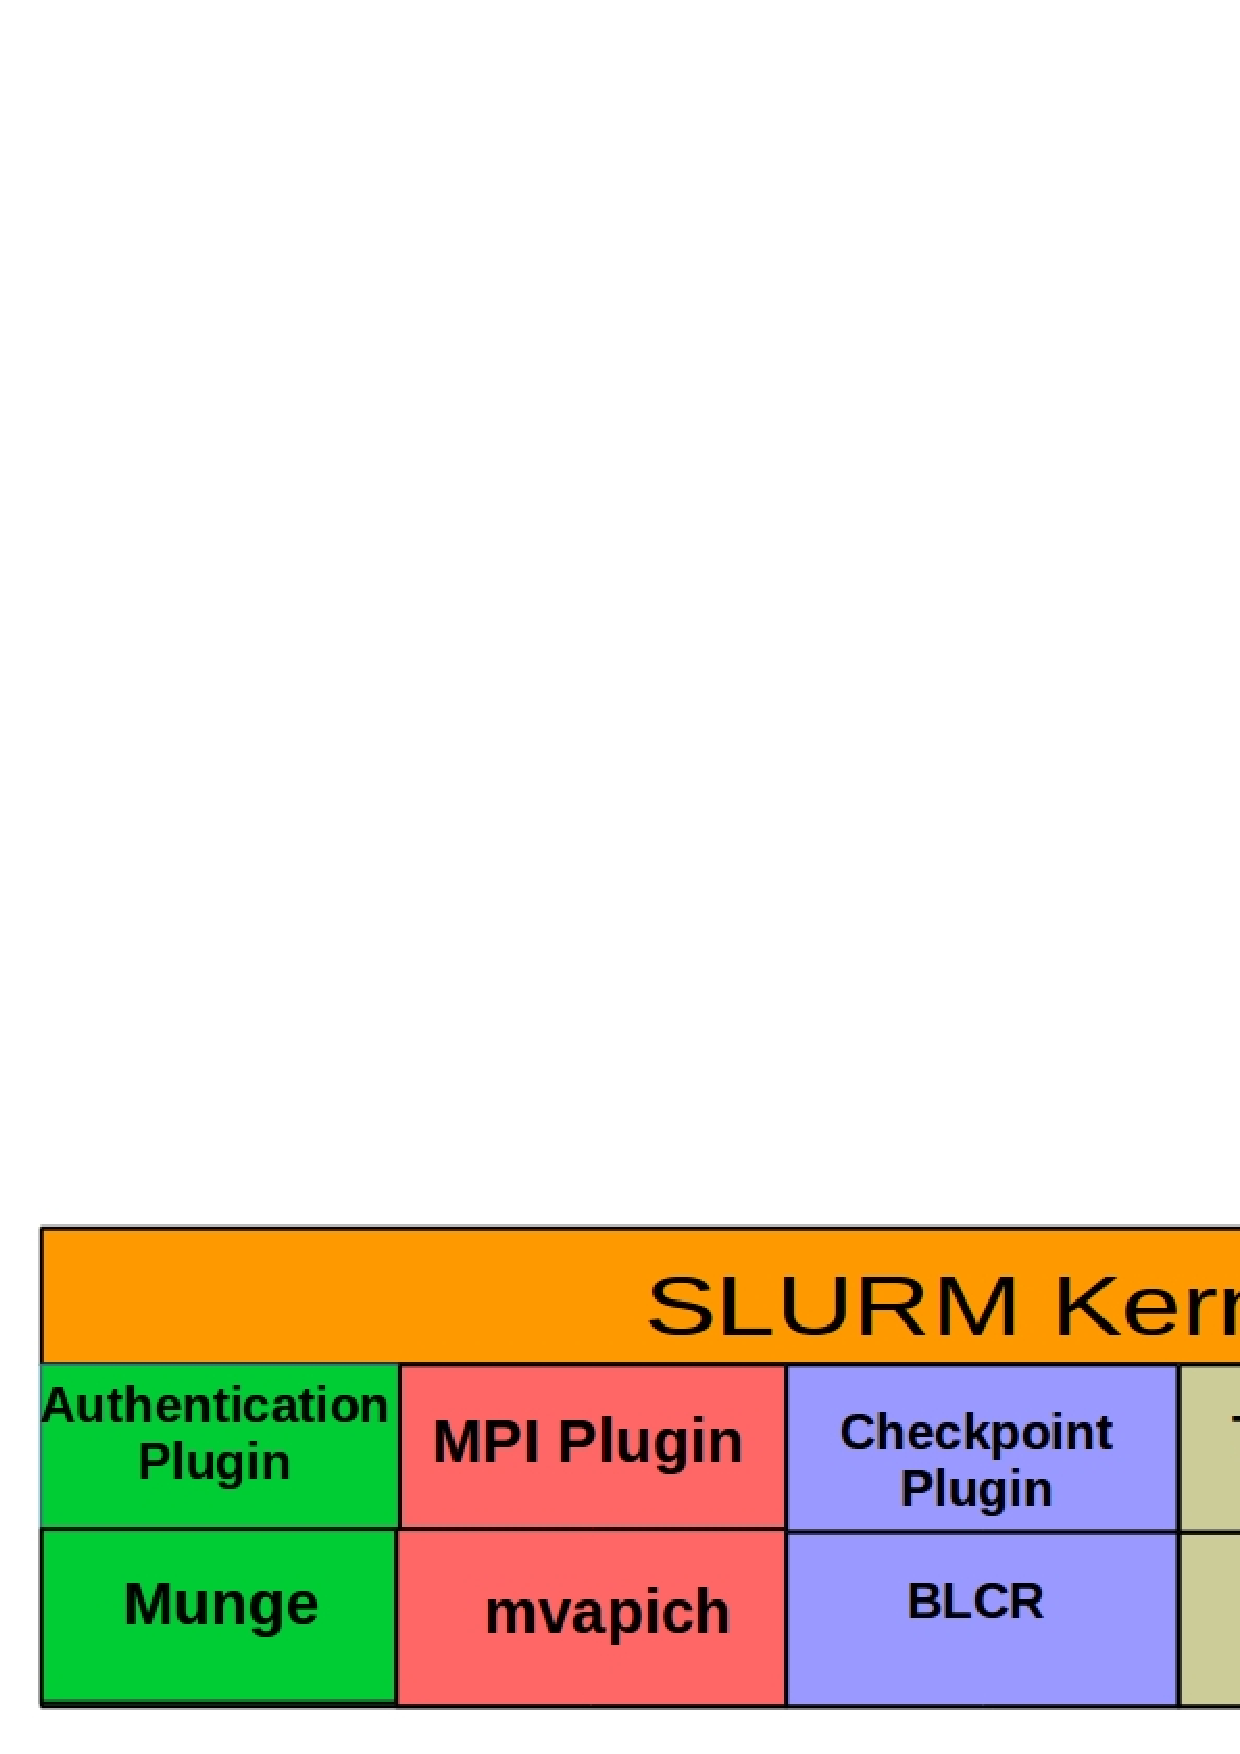
\includegraphics[width=1.0\textwidth]{./figures/plugin.pdf}
%\includegraphics[width=1.0\textwidth]{./figures/plugin.eps}
%\vspace{-0.15in}
%\caption{SLURM with optional Plugins}
%\label{fig:6}
%\end{figure}
%%%%%
\section{Resource Aware Programming}
\subsection{Job Classification}
The throughput of HPC Systems depends not only on efficient job scheduling but also on the type of jobs forming the workload. As defined by Feitelson, and Rudolph\cite{rudolph}, Jobs can be classified into four categories based on their flexibility:
\begin{itemize}
\item \textbf{\textit{Rigid Job:}} Requires a fixed number of resources throughout its execution.
\item \textbf{\textit{Moldable Job: }} The resource requirement of the job can be molded or modified by the batch system before starting the job(e.g. to effectively fit alongside other rigid jobs). Once started its resource set cannot be changed anymore.
\item \textbf{\textit{Evolving Job: }} These kind of jobs request for resource expansion or shrinkage during their execution. Applications that use Multi-Scale Analysis or Adaptive Mesh Refinement (AMR) exhibit this kind of behavior typically due to unexpected increases in computations or having reached hardware limits (e.g. memory) on a node.
\item \textbf{\textit{Malleable Job: }} The expansion and shrinkage of resources are initiated by the batch system in contrast to the evolving jobs. The application adapts itself to the changing resource set.
\end{itemize}
The first two types fall into the category of what is called as the static allocation since the allocation of rigid and moldable jobs must be finalized before the job starts. Whereas, the last two types fall under the category of dynamic allocation since this property of expanding or shrinking evolving and malleable jobs (together termed adaptive jobs) happens at runtime. Adaptive Jobs hold a strong potential to obtain high system performance. Batch systems can substantially improve the system utilization, throughput and response times with efficient shrink/expand strategies for running jobs that are adaptive. Similarly, applications also profit when expanded with additional resources as this can increase application speedup and improve load balance across the job\textquotesingle s resource set.
%%%%%
\subsection{Invasive Programming Models}
In this section, we will briefly look into the details of the earlier invasive extensions done to OpenMP and MPI done as a part of this ongoing research project. This will give us an insight into the earlier approach taken towards realizing such resource-aware programming models. These invasic extensions provide us with a new parallel programming model that allows us to implement resource aware programs. Depending on the semantics of these new extensions, the resulting application can either be evolving(application dictates the changes to its resource set) or a malleable job(resource manager dictates the change in resources to which the application must adapt). Resource awareness could mean that either the program can allocate or free resources according to the amount of available parallelism / the dynamic size of the data or it could mean that it can adapt to the available resources for execution.\\ \\
%%%%%%%%%
Parallel applications that are resource aware will invade or retreat from resources depending on their availability and on the load imbalances encountered during their runtime. To support this, some form of dynamic process management of the parallel application is necessary. And, in order to realize this in practice, the most basic requirement would be the need for a library that will serve as an application programming interface for programmers to implement such invasic applications that are capable of adapting to a changing set of resources. This requirement needs to be complemented by the extension of the resource management systems which would need to allocate / deallocate resources and coordinate with the library to allow for such adaptive operations of an invasive parallel application.\\ \\
\textbf{iOMP}\cite{andreas}\\
The OpenMP parallel programming model for shared memory systems was extended to support the programming of resource aware applications and is named as Invasive OpenMP or iOMP. Parallelization using OpenMP is done by inserting compiler directives into the application's source code to define parallel regions that are executed in parallel by a team of threads whereas the sequential region would be executed by a single master thread. There are different ways to control the number of threads in a parallel region and the most common approach is through the environment variable, or through OpenMP library call or as an additional clause in its directives. iOMP has been implemented as a library in C++ using an object oriented approach and provides two important methods / operations available in its class \textbf{\textit{Claim}}:
%%%%
\begin{itemize}
\item \textbf{\textit{Invade}}: This operation allocates additional resources / PE's (processing elements). A constraint parameter passed as an argument to this operation specifies the details such as which resources and how many of them [range] are additionally required from the resource manager.
\item \textbf{\textit{Retreat}}: This operations deallocates resources / PE's. A constraint parameter passed as an argument to this operation specifies the details such as which resources and how many of them must be freed to the resource manager.
\end{itemize}
%%%%%%
A \textit{Claim} (not the C++ Class) in iOMP refers to all the resources / PE's allocated to the application. This means that an iOMP program will always have a single claim. Initially, the claim size is $1$ but it will increase and decrease during the runtime of the application. The constraint parameter mentioned before also allows the programmer to specify several other constraints such as memory, pinning strategy, architecture specific optimizations etc. Below is a small snippet of code from <ref> that shows an example of iOMP program.
\begin{lstlisting}[frame=single]
int main() 
{
	Claim claim;
	int sum = 0;
	/* Acquire resources according to the given constraints */
	claim.invade(PEQuantity(1, 3));
	
	/* Executing a parallel for loop on the given resources */
	#pragma omp for reduce reduction(+:sum)
	for (int i=0; i < 100000; i++)
		sum += i;
	
	/* Free resources and delete pinning */
	claim.retreat();
}		
\end{lstlisting}
%%%%%%%%
As another important part of the iOMP implementation,  A resource manager has also been implemented. This has a global view of the resources in the shared memory system and acts like a server to every other running application that are its clients. Every client-server communication happens over a message queue. The resource manager handles the redistribution of the resources over time to all running applications based on their invade / retreat operations.\\ \\
%%%%%%%%
%%%%%%%%
\textbf{iMPI}\cite{isaias}\\
Similar to \textbf{iOMP}, previous research effort in this project was also directed towards extending parallel programming models for distributed memory systems. iMPI which stands for Invasive MPI is an extension to the MPI library that can support resource aware programming. The Single-chip Cloud Computer (SCC) from Intel Labs was an experimental CPU that integrates 48 cores and is basically a distributed memory system on the chip. This hardware platform along with its interesting memory features was used in order to evaluate this invasive programming model.\\ \\
%%%%%%
Message Passing has for long remained the dominant programming model for distributed memory systems. MPI stands for Message Passing Interface. It is a standardized and portable message passing system designed to function on a wide variety of parallel computers. It implements a message passing type of parallel programming model where the application consists of a set of processes with separate address spaces. The processes exchange messages by explicit send/receive operations. The following are the invasive extensions to MPI:
\begin{itemize}
\item \textbf{\textit{MPI\_Comm\_invade}}: The main purpose of this operation is to reserve resources and for this it looks into what resources are currently available and invades them.
\item \textbf{\textit{MPI\_Comm\_infect}}: This operation is used by the application to specify the total number of cores to infect and which ones are preferred. This number can be less than or equal to the total number of cores that were reserved by the invade operation. 
\item \textbf{\textit{MPI\_Comm\_retreat}}: This operation does the reverse of the invade+infect sequence. Instead of reserving and claiming resources, it returns them so that other invasive applications can claim them.
\end{itemize}
The above extensions were based on the MPICH2 library. A new process manager called \textbf{Invasive Process Manager (IPM)} was also developed as a part of the iMPI implementation. It was responsible for launching of the MPI jobs, as well as spawn operations (invade+infect) with low latency and functionality for resource awareness.\\ \\
\textbf{Other Resource-Aware Programming Models} <TBA> <Do not know if this is needed and instead can be in the related work section>
%%%%%%%%%
%%%%%%%%%
\section{Invasive Resource Management}
In this section, we will look at the latest extensions done to the MPI library for programming on HPC systems like clusters, supercomputers etc and also the extensions required for resource managers managing these HPC systems. This is in contrast to the earlier version of the iMPI which was targeted towards the Intel SCC platform. The MPI and Resource Manager extensions are not accomplished as a part of this thesis but are essential to be described here in order to get the right context for adaptive applications and their scheduling.
\subsection{Invasive MPI}
Traditionally MPI applications are static in nature which means that they are executed with a fixed number of processes. Dynamic process support is available through MPI spawn and its related operations. MPI spawn operation creates child processes in a separate child process group and thereafter both the parent and child process groups are connected by an intercommunicator. Many drawbacks of this dynamic process functionality have motivated the need for such an extended programming model. Some of these drawbacks are: spawn is a collective operation across the parent and child process group, intercommunicators complicate development effort as more spawn operations create more disjoint process groups, destruction of entire process groups is the only option limiting the granularity and location of releasing resources, spawn usually operates within the same unmodified resource allocation.\\ \\
%\noindent
%%%%%%%%
To overcome these drawbacks, Invasive MPI is being developed as an extended version of the MPI library that provides new API calls in order to allow the programmer to create an invasive MPI application. These extensions are necessary to make the application resource aware and to adapt according to a change in the resource set by performing data / load redistributions. Following are the proposed extensions being implemented in MPICH:\\ \\
%\begin{itemize}
%\item 
\textbf{\textit{MPI Initialization in Adaptive Mode}} This allows the application to be initialized in adaptive mode. It is an extension of the standard MPI{\_}Init operation and is now called as MPI{\_}Init{\_}adapt. The difference now is that a new parameter called local status is being passed. Upon the return of this Init function, local status will hold a value of \textit{new} if the process doing this MPI initialization was created using the mpiexec command or it will hold a value of \textit{joining} if the process was created by the resource manager as a part of the expansion of an already running invasive MPI application. The \textit{joining} processes will then begin an adaptation window after completing the initialization. 
\begin{lstlisting}[frame=single]
int 
MPI_Init_adapt( int *argc,
                char ***argv,
                int *local_status,
              );
\end{lstlisting}
%\item 
\textbf{\textit{Probing Adaptation Data}} The resource manager decides when and how the adaptation of a running application will be initiated. This operation will allow the application to probe the resource manager for adaptation instructions. This operation is called MPI{\_}Probe{\_}adapt and instructs the application on whether there is an adaptation pending.  
\begin{lstlisting}[frame=single]
int
MPI_Probe_adapt( int *current_operation,
                 int *local_status,
                 int *nfailed,
                 int *failed_ranks,
                 MPI_Info *info
               );
\end{lstlisting}
A value of false returned from the current operation parameter will simply tell the application to continue doing progress normally. A true or fault value indicates that there is an adaptation to be done. In the case of a fault, the application will receive information of the failed MPI ranks, since failed processes may no longer be reachable. This operation will also provide the application with additional information on whether it is a joining process if the process was created by the resource manager to represent newly allocated resources as a part of an expansion operation. Joining processes can skip calling the probe operation. If the information returned is staying then it means it should remain in the process group after the adaptation, otherwise it is retreating.\\ \\
%\item 
\textbf{\textit{Beginning an Adaptation Window}} This operation marks the start of an adaptation window. It provides two communicators as output: one intercommunicator that is equivalent to what is provided by standard spawn operations, and one intracommunicator that gives an early view of how the MPI{\_}COMM{\_}WORLD communicator will look like after the adaptation is committed. It is up to the application to make calls to this operation in a safe location. Each process is required to read its future rank and the future  size of the process group from the helper new{\_}comm{\_}world communicator to perform an adaptation consistently. This new size and local rank of the process will persist after the MPI{\_}COMM{\_}ADAPT{\_}COMMIT operation. Processes that are retreating during the adaptation window will not have access to the future MPI{\_}COMM{\_}WORLD, since a retreating process will be removed from the process group, their new{\_}comm{\_}world will be set to MPI{\_}COMM{\_}NULL. These processes will need to be reached over the provided intercomm from the children, or their current MPI{\_}COMM{\_}WORLD from the parents, during the adaptation window.
\begin{lstlisting}[frame=single]
int
MPI_Comm_adapt_begin( 
         MPI_Comm *intercomm,
         MPI_Comm *new_comm_world,
         );
\end{lstlisting}
%\item 
\textbf{\textit{Commiting an Adaptation Window}} This operation commits the adaptation. This operation affects MPI{\_}COMM{\_}WORLD: any process that has retired is eliminated from it, and any new joining process is inserted into it. After the commit, the MPI{\_}COMM{\_}WORLD communicator will match exactly the new{\_}comm{\_}world intracommunicator provided by the previously mentioned MPI{\_}COMM{\_}ADAPT{\_}BEGIN operation. This operation also notifies the resource manager that the current adaptation is complete.
\begin{lstlisting}[frame=single]
int
MPI_Comm_adapt_commit(); 
\end{lstlisting}
%\end{itemize}
\subsection{Resource Management Extensions}
Existing batch systems usually support only static allocation of resources to applications before they start. We need to integrate invasive resource management into these existing batch systems in order to change the allocated resources dynamically at runtime. This will allow for an elastic execution of MPI applications. Such efforts have already been initiated in the Flux project\cite{schulz}. Existing systems like SLURM allow a job to have extra resources by expanding its allocation. But, this does not fully satisfy the use case here as we need to either grow or shrink the application. Another important factor is the support needed from a programming model that would allow applications to be adaptive to such allocations. The extensions needed on the MPI library side have already been mentioned in the previous section. In order to achieve the extensions on the resource manager side the following SLURM components have been extended:\\ \\
%\begin{itemize}
%\item
\textbf{SLURM}\\
The resource manager needs to closely coordinate with the invasive MPI library to support invasive applications. It needs to fork processes on new resources when an application is expanding or destroy them in case it is shrinking. Both of which needs to be done in coordination with MPI. New processes could be created in the existing resource allocation of the running application, possibly allowing for oversubscription of CPU cores, but that would be of little benefit to most HPC application's performance and scalability. The following are the extensions specific to SLURM. Figure \ref{fig:1} shows an example of job adaptation using the below extensions.\\ \\
%\begin{itemize}
%\item 
\textbf{\textit{Slurmctld Extensions}} A new operation that initiates an adaptation through the \textit{srun} command: \textit{srun{\_}realloc{\_}message} is introduced. This message is sent by slurmctld to the srun responsible for this job. The \textit{srun{\_}realloc{\_}message} provides \textit{srun} the following information: the list of new nodes allocated to the application and the number of processes to create on them, the list of nodes from where processes need to be destroyed and how many processes to destroy in them, the full list of nodes that compose the new allocation, and other necessary details. Currently adaptations are based on full nodes but future developments will support fine grain scheduling. When a transformation is triggered on a job, its status changes from \textit{RUNNING} to \textit{ADAPTING}. Each application notifies the resource manager when its adaptation is completed and its job record will get updated from the status \textit{ADAPTING} to \textit{RUNNING}; this state change marks the application as eligible for adaptations again and its released resources available for other jobs.\\ \\
%\item 
%\begin{figure}[!htbp]
\begin{figure}[t]
\vspace{-0.60cm}
%\centering
%\includegraphics[width=1.0\textwidth, height=185mm]{./figures/"software architecture".pdf}
\includegraphics[width=1.0\textwidth, height=100mm]{./figures/"RMExtensions".pdf}
\caption{Job Adaptation Flow}
\label{fig:1}
\end{figure}
\textbf{\textit{Slurmd Extensions}} In order to support the MPI{\_}Probe{\_}adapt operation, the PMI plugin for PMI2 interface towards MPI applications has been extended. This plugin is loaded by slurmd daemon after it starts up. The extensions are: Notifying the local daemon that joining processes are waiting in the MPI{\_}Comm{\_}adapt{\_}begin operation, Notifying the local daemon that both the joining and preexisting processes have completed their adaptation and exited MPI{\_}Comm{\_}adapt{\_}commit. The first extension to the PMI is used by the leader process of the joining group. It notifies its local Slumd daemon, which then notifies the srun instance of the job step. The Srun instance then proceeds to notify each of the Slurmd daemons running in the preexisting nodes. These daemons then proceed to update their local MPI{\_}Probe{\_}adapt metadata. The second extension to the PMI is used by the leader process of the new adapted process group, that was created as a result of a successful completion of MPI{\_}Comm{\_}adapt{\_}commit. The local daemon sends a notification message to Srun, which then forwards it to Slurmctld. The controller handles this message by updating the status of the job from \textit{JOB{\_}ADAPTING} to \textit{JOB{\_}RUNNING}.\\ \\
%item
\textbf{\textit{Srun Extensions}} Most of the operations that are initiated by either the controller or any application process (via the PMI and the SLURMD daemons) is handled partially by srun. It will handle the reallocation message received from the controller, notification that joining processes are ready and waiting in the MPI{\_}Comm{\_}adapt{\_}begin operation, notification that the adaptation was completed though a successful MPI{\_}Comm{\_}adapt{\_}commit. In addition to these handlers, srun has also been extended to manage the IO redirection of joining processes. In the original implementation, these were setup only at launch time; it can now manage redirections dynamically as processes are created and destroyed.

\chapter{Dynamic Resource Management Architecture["What we are building". Abstraction of the complete system at a high level showing all the components and how they will interact with each other like a skeleton. It deals with what is being done and where is it being done but not how. The "how" is tackled in the design}\label{chapter:dynamic resource}

\section{System Design}

This section illustrates and describes a high level design of the software implemented with the help of protocol sequence diagrams and state machine diagrams. It will help to understand at a high level as to how the system has been designed to support this new approach of invasive computing and how will many of its components in the software hierarchy interact with each other with new protocols or extensions of existing protocols to integrate such an invasive resource management into current batch systems.\\

The following page shows the software architecture of how Invasive Resource Management can be supported with a traditional resource manager and how exactly the new software components will fit in the existing software hierarchy. The \ref{fig:7} relates closely to how SLURM is organized since the intention of this work would be to demonstrate the support for Invasive Computing with the help of SLURM as a resource manager.
\begin{itemize}
\item The top layer is that of the core resource management component which has access to job queues. In this architecture, it will now have access to not only the queue for the legacy(static) jobs but also invasive job queue(jobs submittted to invasic partition that supports invasive computing).
\item In a traditional setup the top layer will perform the task of job scheduling as well. This means that it will select a job(s) from the queue of jobs based on the current state of resources and many other factors to dispatch it to the traditional process manager below in the hierarchy. The process manager then takes the responsibility of launching these jobs on the allocated resources in the partition and managing them for their full lifetime. In case of parallel jobs, it will manage the job in a parallel environment along with facilitating the communication amongst the parallel tasks/processes with the help of a PMI(Process Manager Interface) server. The process manager may also spawn slave daemons on each of the nodes which are a part of the resource allocation for a single job to manage them more effectively.
\item As discussed in the previous chapter, an independent Invasive resource management component by the name "iHypervisor" will be implemented which needs to communicate with a new scheduling component iScheduler and influence the scheduling decisions taken by it. The iHypervisor sits between the top layer and the process manager.
\item A new job scheduler specifically for invasive jobs needs to be integrated into the existing batch system. This is due to the reason that the scheduler for invasive jobs will work in a different manner based on the approach described earlier in comparison to the legacy job scheduler for static jobs. In case of SLURM which has a modular design with several optional plugins, a new plugin by name "iScheduler" will be implemented for SLURM to handle job scheduling specifically for invasic jobs.
\item Communication between iHypervisor and iScheduler will involve the negotiation protocol as explained in the previous chapter but will also include periodic feedbacks being sent by iHypervisor to iScheduler having some useful statistical measures about current state of resources, resource utilization, job throughput etc. that may help influence the decision making of iScheduler. This communication will also additionally support a means to service urgent jobs immediately.
\end{itemize}
\begin{figure}[!htbp]
\centering
%\includegraphics[width=1.0\textwidth, height=185mm]{./figures/"software architecture".pdf}
\includegraphics[width=1.0\textwidth, height=185mm]{./figures/"software architecture".eps}
\caption{Invasive Resource Management Architecture}
\label{fig:7}
\end{figure}
\begin{figure}[h]
\centering
%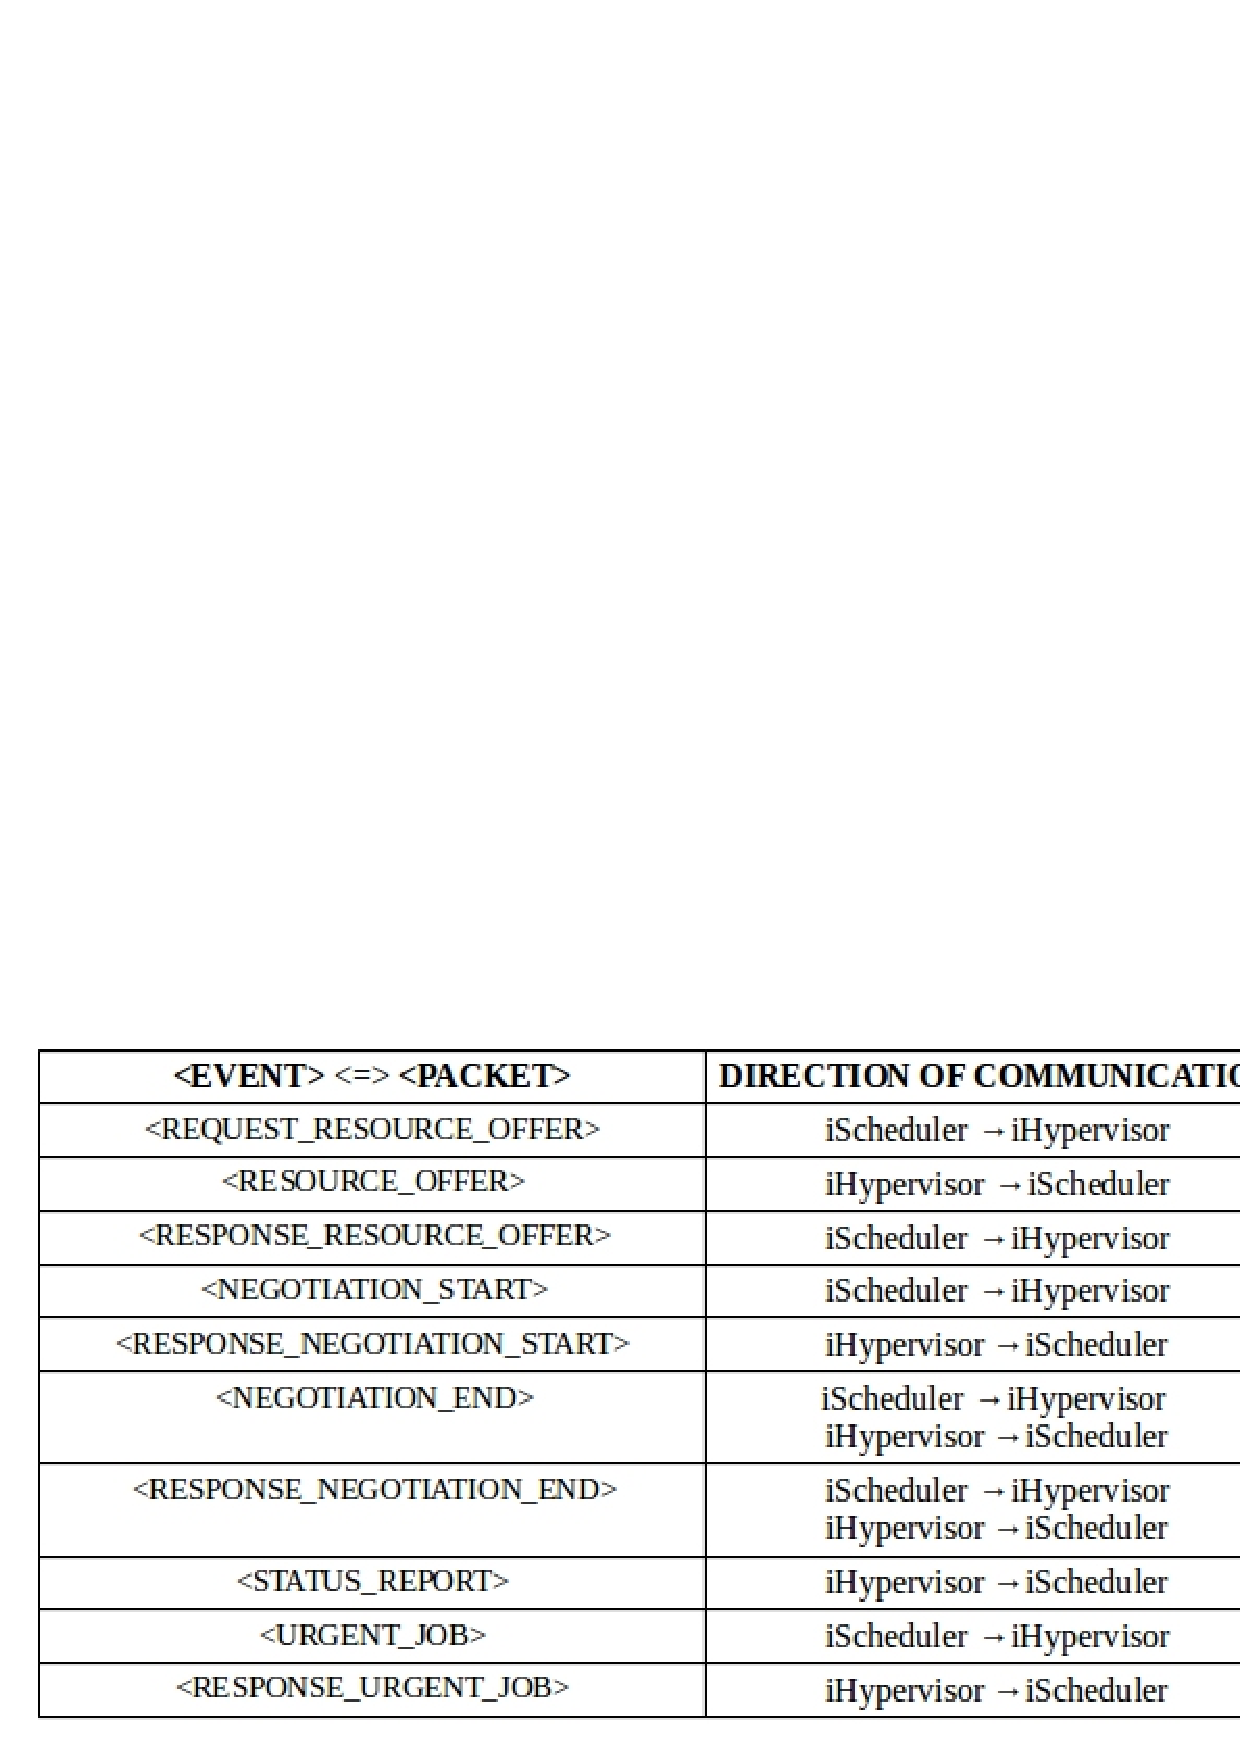
\includegraphics[width=1.0\textwidth, height=80mm]{./figures/table.pdf}
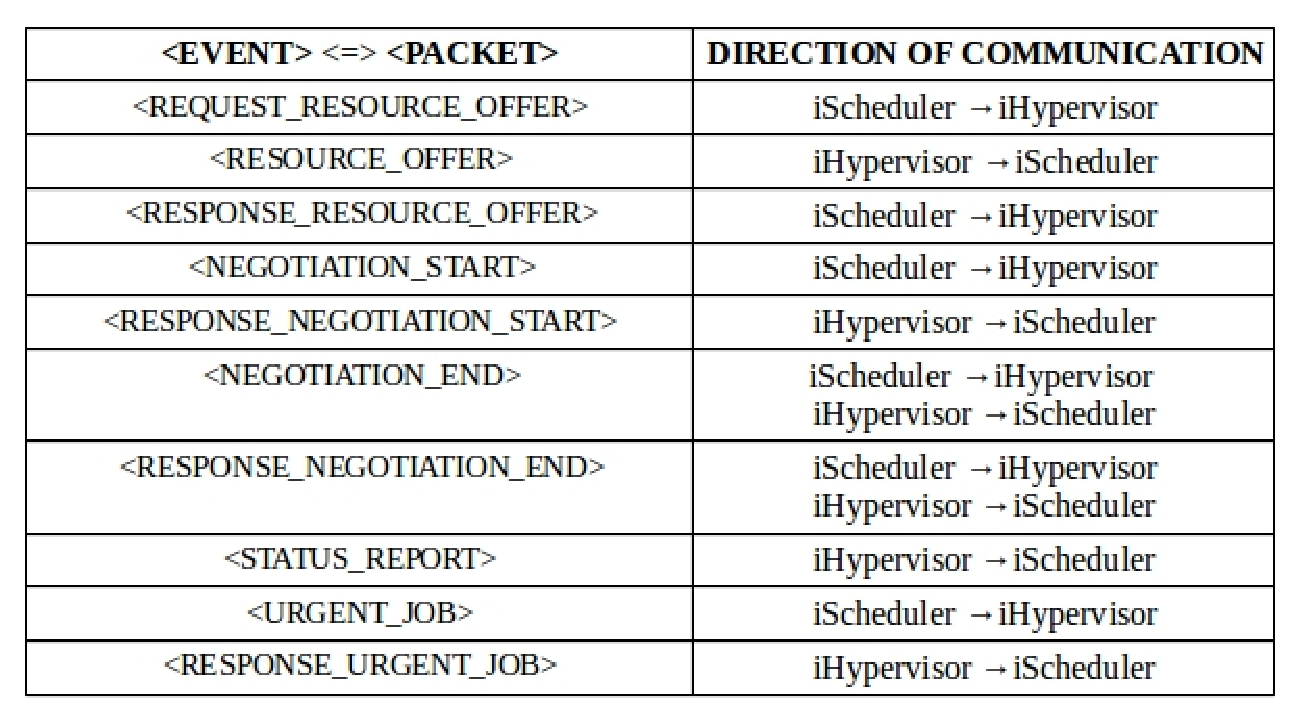
\includegraphics[width=1.0\textwidth, height=80mm]{./figures/table.eps}
\caption{Message Types}
\label{fig:8}
\end{figure}

\textbf{Communication Phases}
\begin{itemize}
\item \textbf{\textit{Protocol Initialization:}} This phase basically establishes the initial environment between the communicating parties (iScheduler and iHypervisor) for proper communication later on. Successful initialization of this phase prepares both the parties to start negotiating based on the negotiation protocol described in the following points. During this protocol initialization various parameters such as protocl version, maximum attempts for negotiation, timer intervals and several others could be exchanged to set up the internal data structures and configuration tables for both the communicating parties. This protocol is a bi-directional communication.
\item \textbf{\textit{Protocol Finalization:}} This phases signals the end of communication between iHypervisor and iScheduler using negotiation protocol. It leads to a safe termination of this communication followed by the release of any internal data structures allocated earlier along with configuration parameters. This results in consistent behaviour of both the communicating parties which can then proceed to safely terminate and exit. This protocol is a bi-directional communication.
\item \textbf{\textit{Negotiation:}} This is the most important phase in this whole approach to support invasive computing as discussed in the previous chapter. It is the phase during which both iHypervisor and iScheduler are negotiating with each other till they reach an agreement. If they do not then they continue till a certain limit to the number of negotiating attempts are reached after which both of them just agree in their final attempt closing the current negotiation. After this a new transaction of negotiation begins.
\item \textbf{\textit{Feedback:}} This concerns the periodic feedback sent by the iHypervisor to the iScheduler containing useful information such as the job states, latest snapshot of the resources in the invasic partition and many other statistical measures not limited to system utilization, job throughput, waiting times of jobs to help and influence the iScheduler in its decision making for scheduling jobs during its future transactions of negotiation. This protocol is a uni-directional communication.
\item \textbf{\textit{Urgent Jobs:}} This protocol concerns the support for urgent jobs. At any given point of time a cluster or supercomputing center may want to support very high priority jobs immediately without any further delay. By introducing support for invasive computing, it makes it all the more feasible to help run these urgent jobs immediately by either shrinking the resources of other jobs or suspending/Killing them.
\end{itemize}

\textbf{\textit{Separation of Concerns: }}In this thesis, The idea of separating the batch and runtime scheduling components of a Job Scheduler is explored. 

\subsection{Invasive Batch Scheduler}
Today almost all resource management systems fall into the category of queuing systems. Several queues with different limits on the number of requested resources and the duration exist for the submission of resource requests. Jobs within a queue are ordered according to a scheduling policy, e. g. FCFS (first come, first serve). Queues might be activated only for specific times (e. g. prime time, non prime time, or weekend). The task of a queuing system is to assign free resources to waiting requests. The highest prioritized request is always the queue head. If it is possible to start more than one queue head, further criteria like queue priority or best fit (e. g. leaving less resources idle) are used to select a request. There might also exist a high priority queue whose jobs are preferred at any time. If not enough resources are available to start any of the queue heads, the system waits until enough resources become available. These idle resources may be utilized with less prioritized requests by backfilling mechanisms.
\subsection{Invasive Run Time Scheduler}
\subsection{iMPI Process Manager}


\section{Negotiation Protocol}
\subsection{Protocol Sequence Diagrams}
\vspace{-0.15in}
\begin{figure}[!htbp]
%\begin{figure}[H]
\centering
%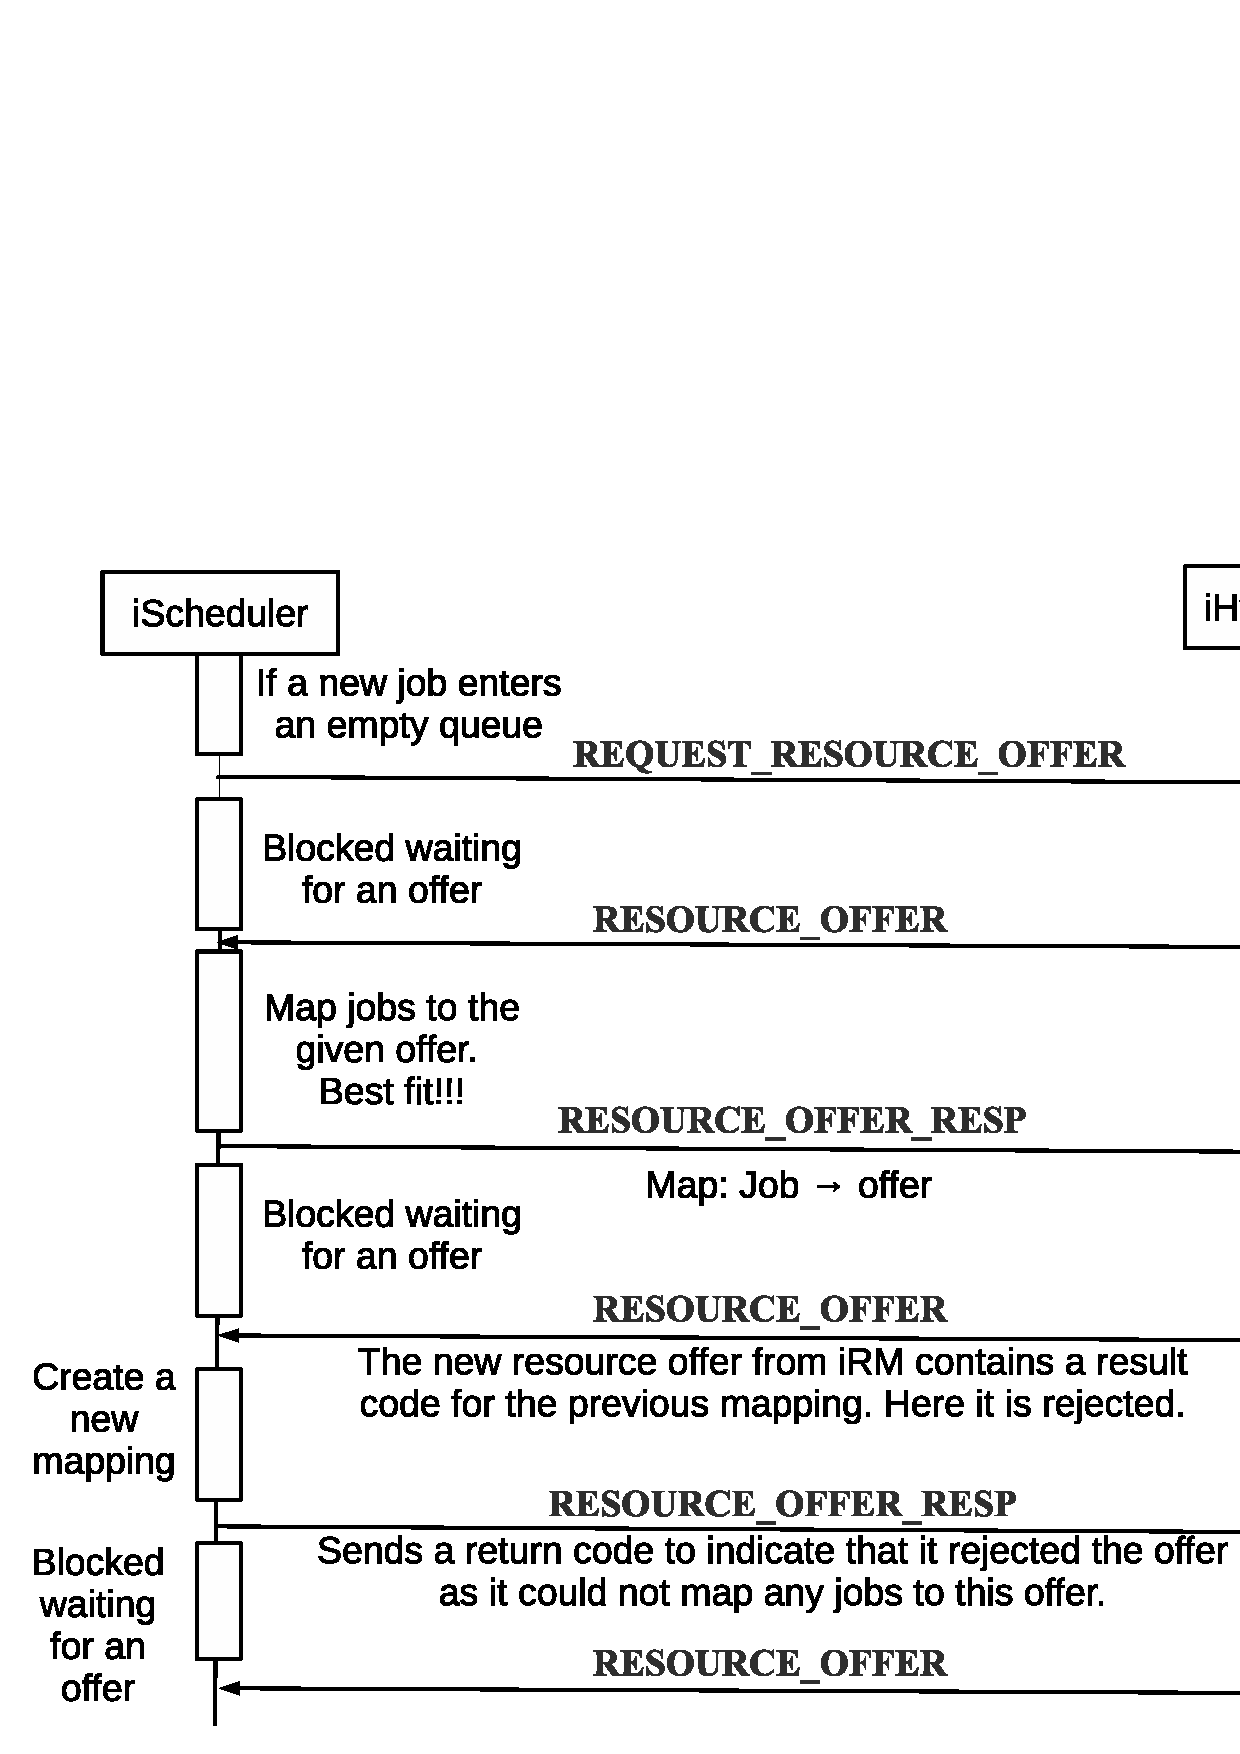
\includegraphics[width=1.0\textwidth, height=100mm]{./figures/figures.pdf}
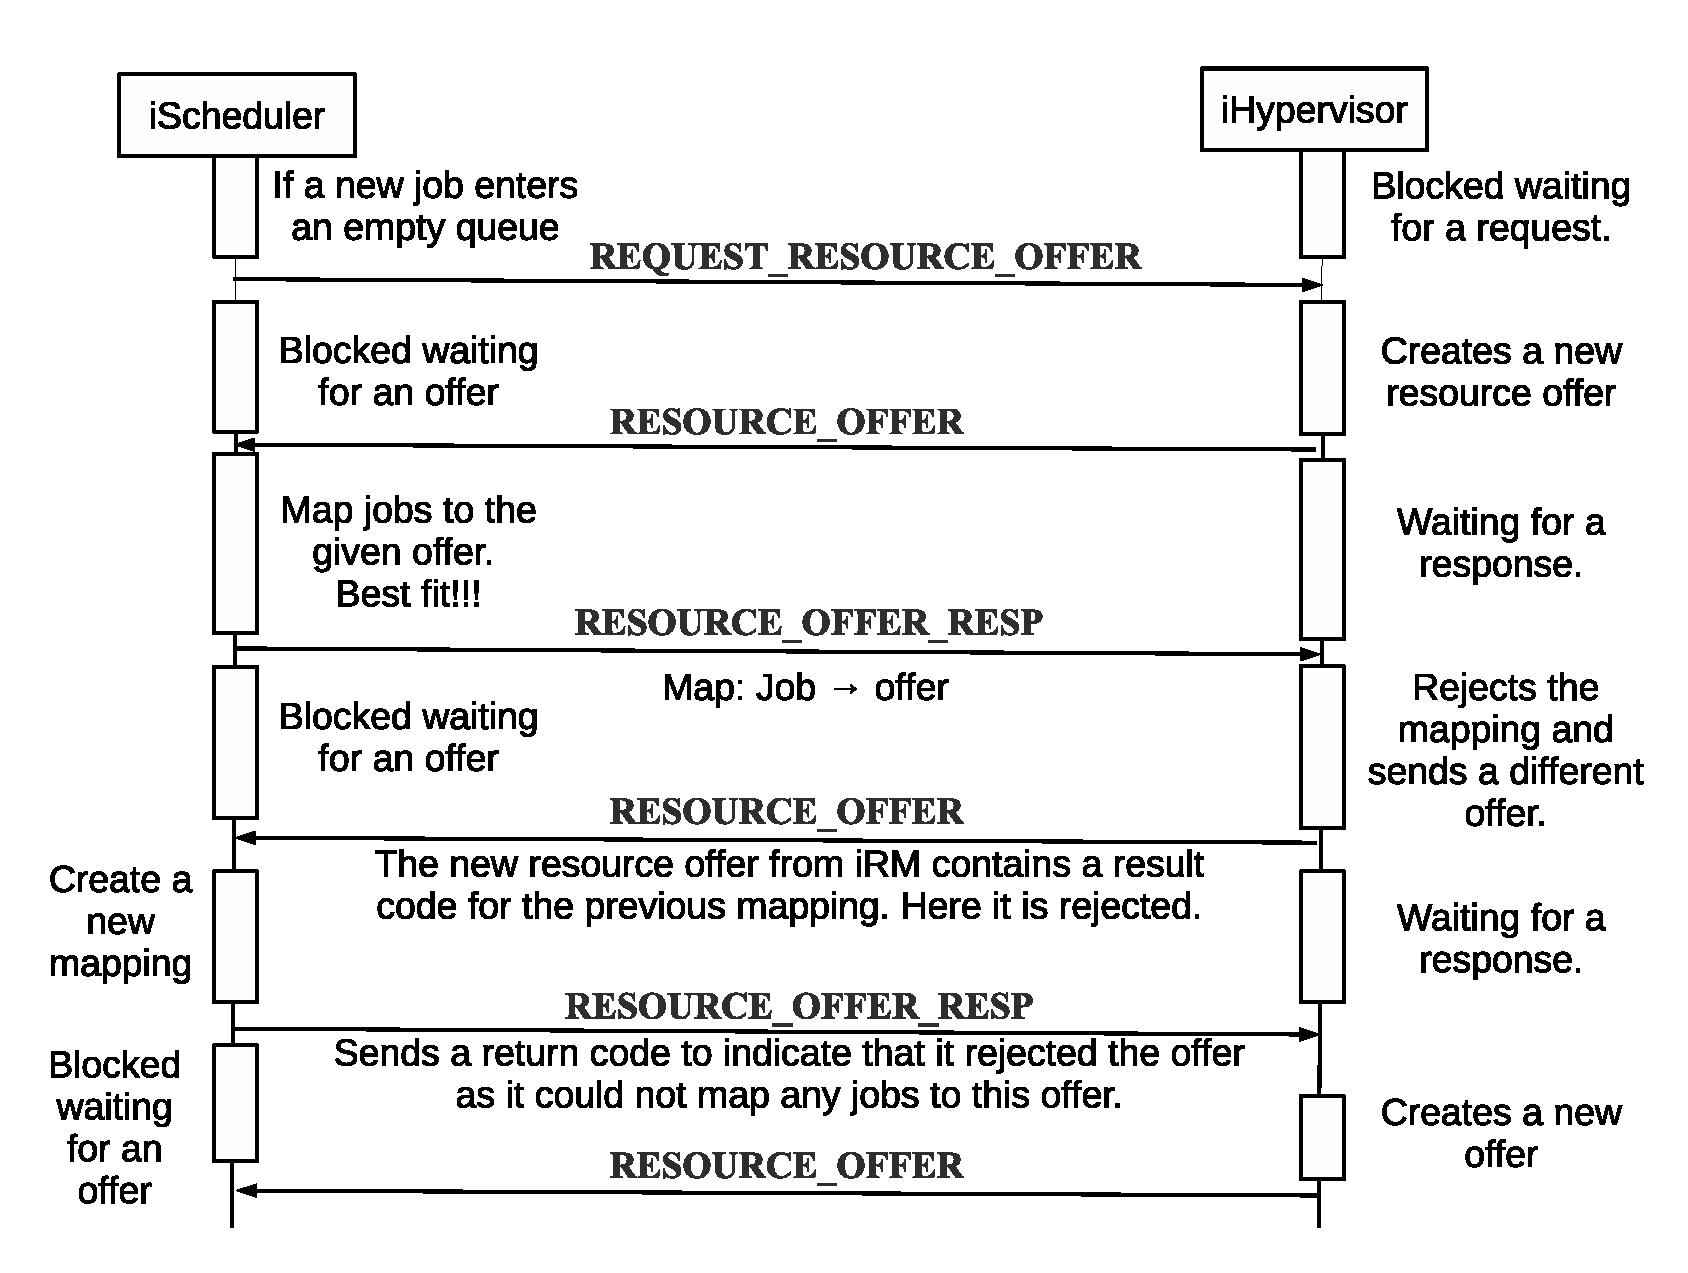
\includegraphics[width=1.0\textwidth, height=100mm]{./figures/figures.eps}
\caption{Scenario 1}
\begin{itemize}
\item Above diagram illustrates a scenario where both iScheduler and iHpervisor are negotiating with each other. The scenario is continued in the next page. \ref{fig:Seq2} illustrates another scenario where negotiations may stop when job queue becomes empty and iHypevisor then will wait for a request from iScheduler for a resource offer that will happen when new jobs arrive.
\item iScheduler makes scheduling decisions at a coarser level of granularity which is nodes whereas iHypervisor does at the granularity of cores and sockets. Both will negotiate with each other till they reach an agreement.
\item It is an event based scheduling which means iScheduler makes a scheduling decision only when it is triggered by receiving a resource offer from iHypervisor. It is only at the start when there are no jobs in the queue and during the operations when the queue may become empty that the iScheduler will have to explicitly send a request message to iHypervisor for a resource offer otherwise at all other times scheduling is event based.
\end{itemize}
\label{fig:Seq1}
\end{figure}
\vspace{-0.25in}
\begin{figure}[!htbp]
\centering
%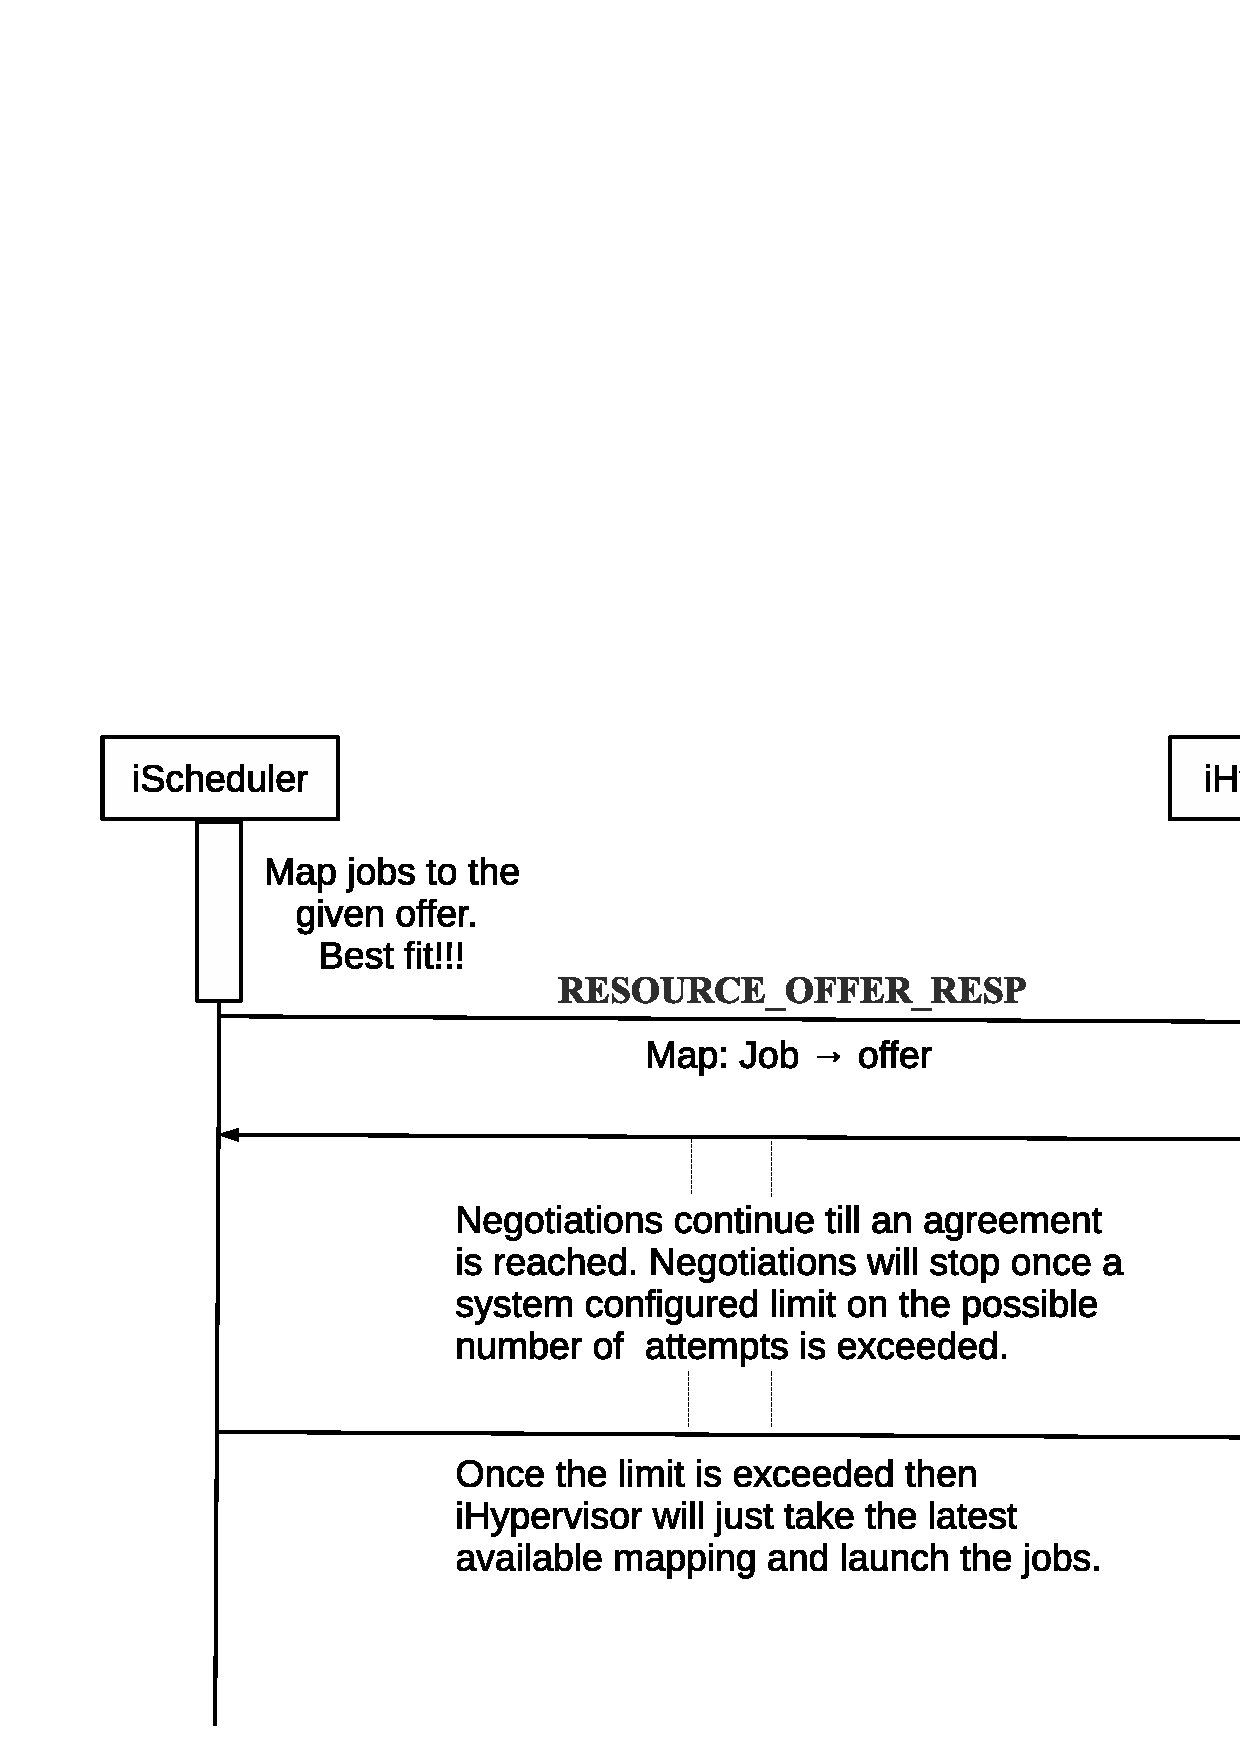
\includegraphics[width=0.9\textwidth, height=100mm]{./figures/figures1.pdf}
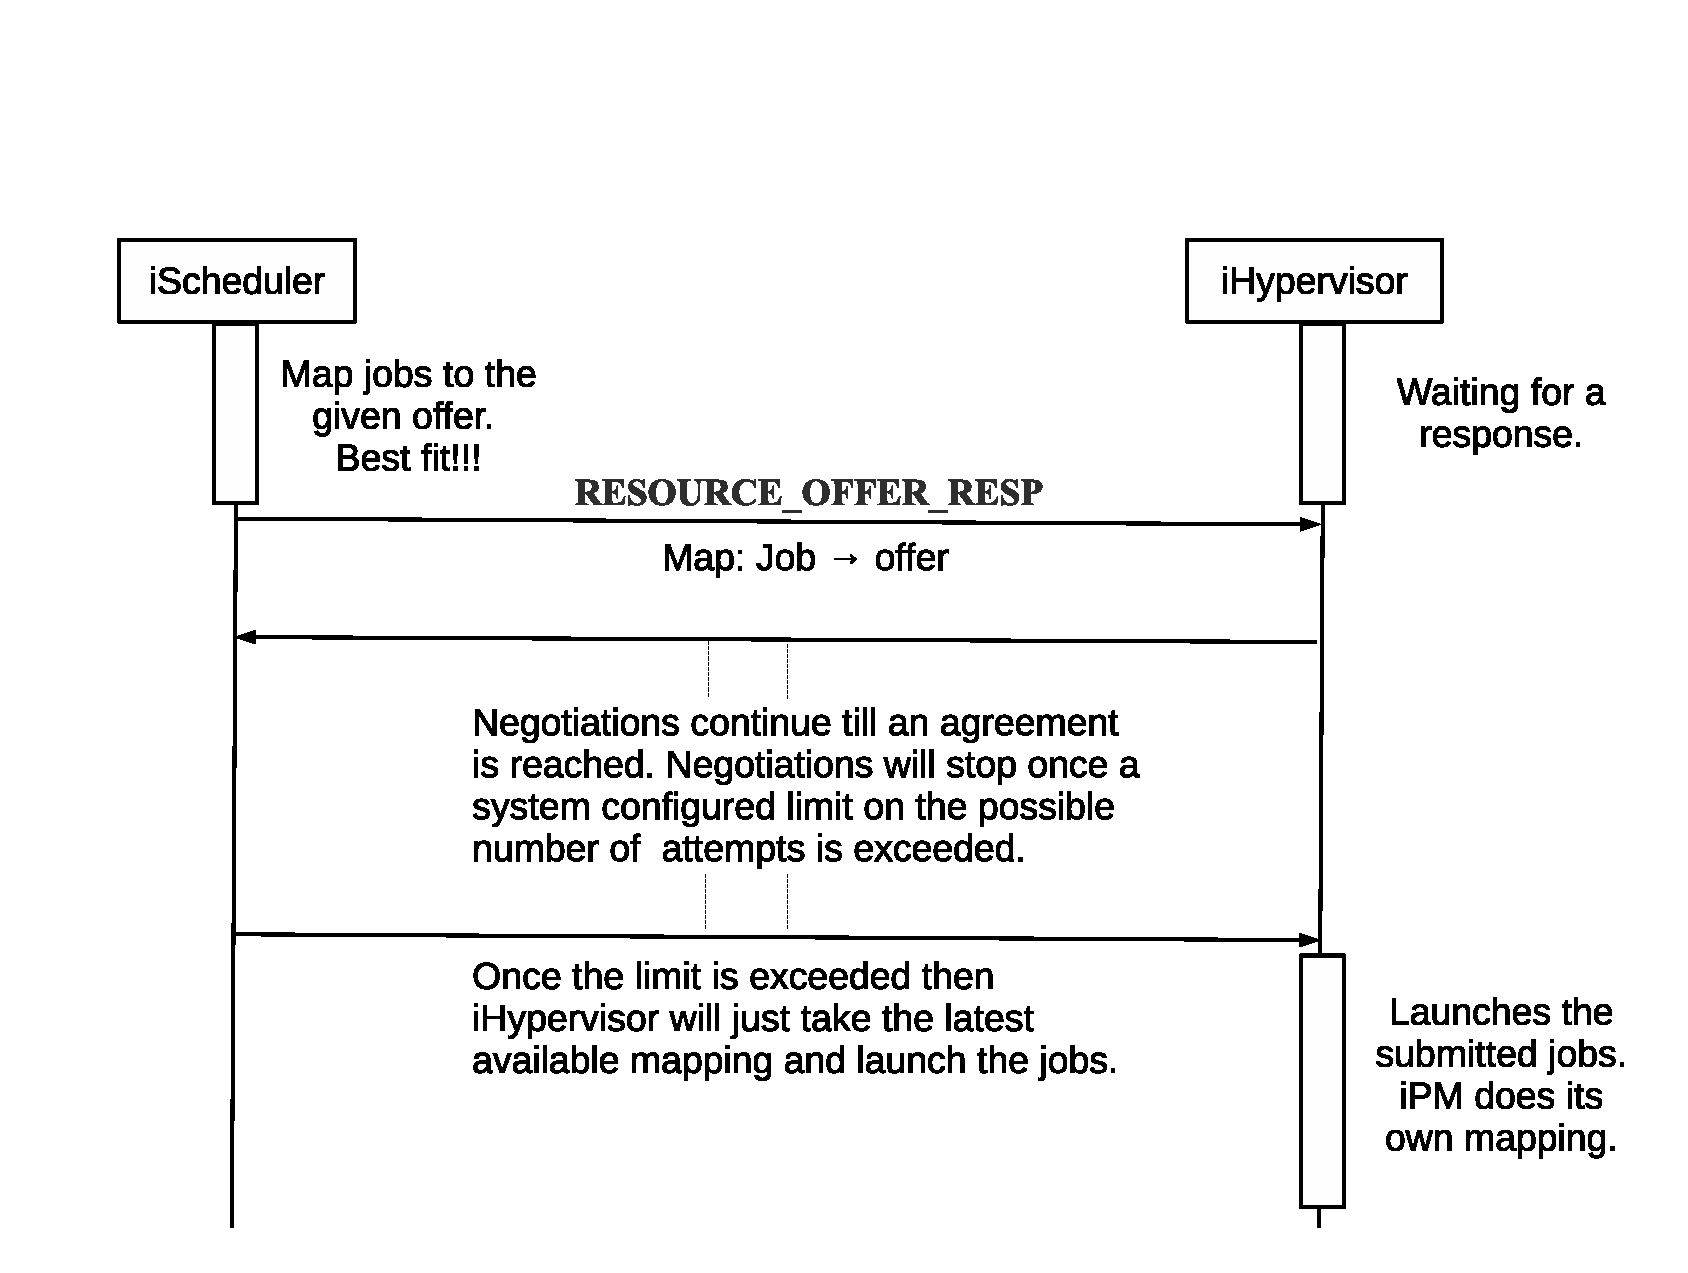
\includegraphics[width=0.9\textwidth, height=100mm]{./figures/figures1.eps}
\caption{Scenario 1 contd.}
\label{fig:Seq1}
\vspace{0.25in}
%\end{figure}
%\begin{figure}[b]
\centering
%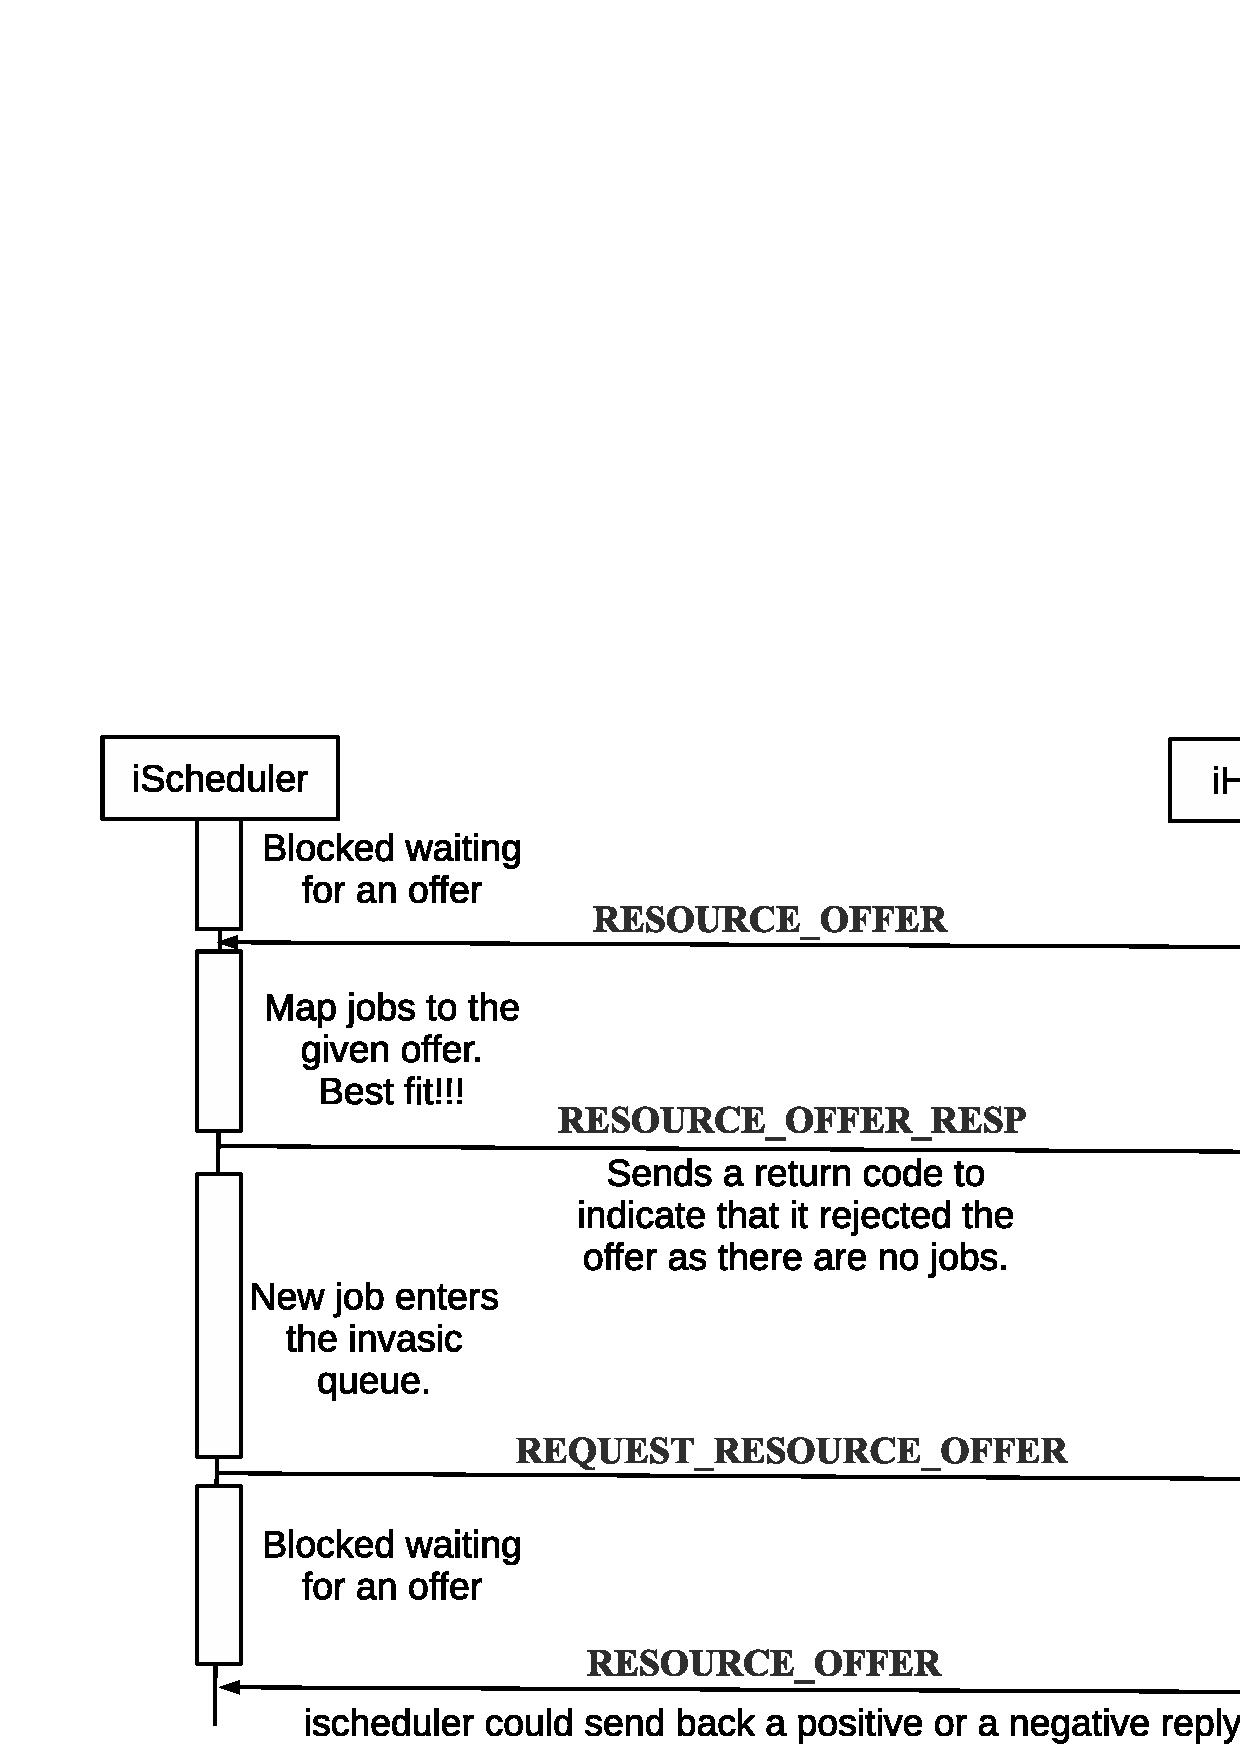
\includegraphics[width=0.9\textwidth, height=100mm]{./figures/figures2.pdf}
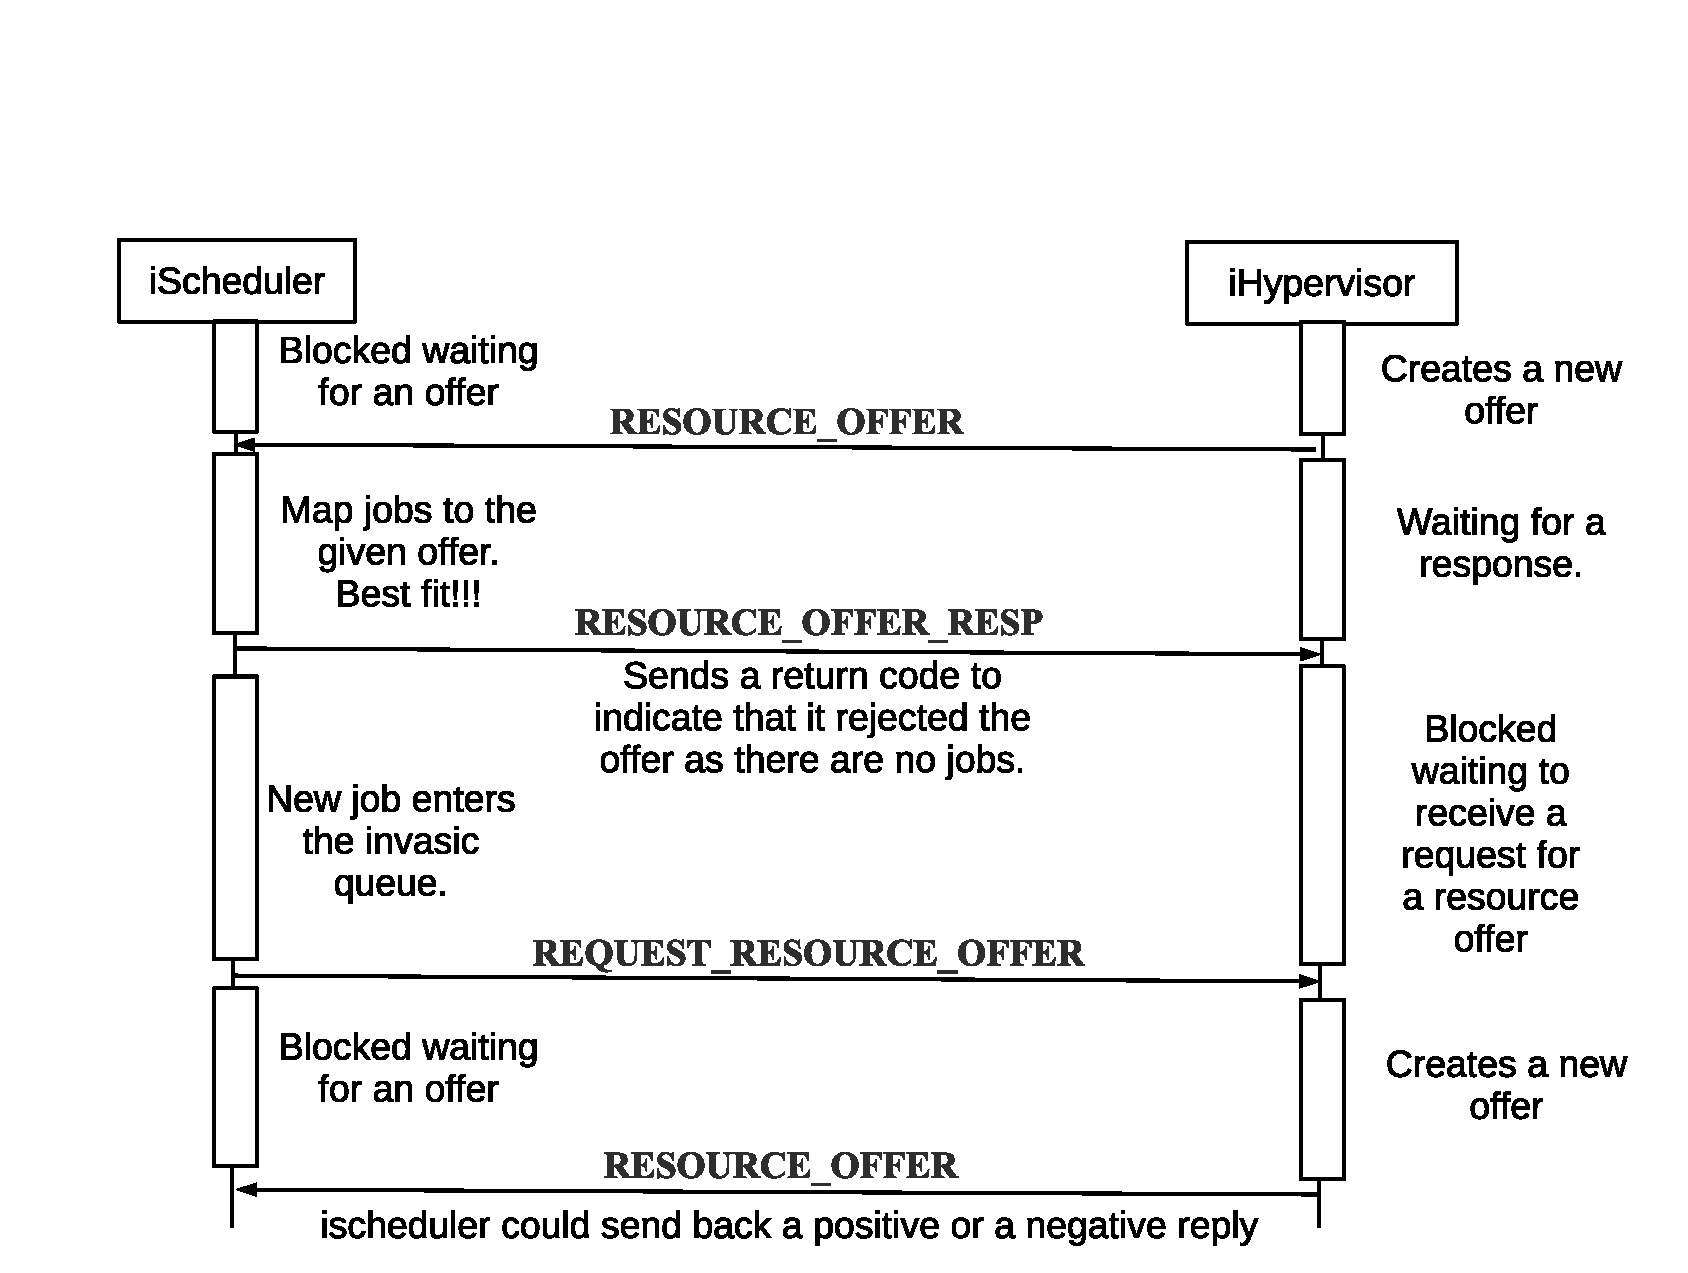
\includegraphics[width=0.9\textwidth, height=100mm]{./figures/figures2.eps}
\caption{Scenario 2}
\label{fig:Seq2}
\end{figure}
%\subsection{State Machine Diagrams}
This section focuses on iScheduler and a thread iRM\_AGENT that it spawns which is the one responsible for all the communication with the iHypervisor including spawning other agent threads for handling feedbacks and urgent jobs.
\vspace{10mm}
\begin{figure}[h]
\centering
%\includegraphics[width=1.0\textwidth, height=150mm]{./figures/"iRM Agent".pdf}
\includegraphics[width=1.0\textwidth, height=150mm]{./figures/"iRM Agent".eps}
\caption{iRM Agent}
\label{fig:Init}
\end{figure}
\begin{itemize}
\item Above diagram and the ones in the following pages illustrate state machine diagrams for few of the communication phases described earlier starting first with a general diagram of how the mulithreaded component iRM agent inside iScheduler starts up and shuts down.
\end{itemize}
\vspace{-20mm}
\begin{figure}[h]
\centering
%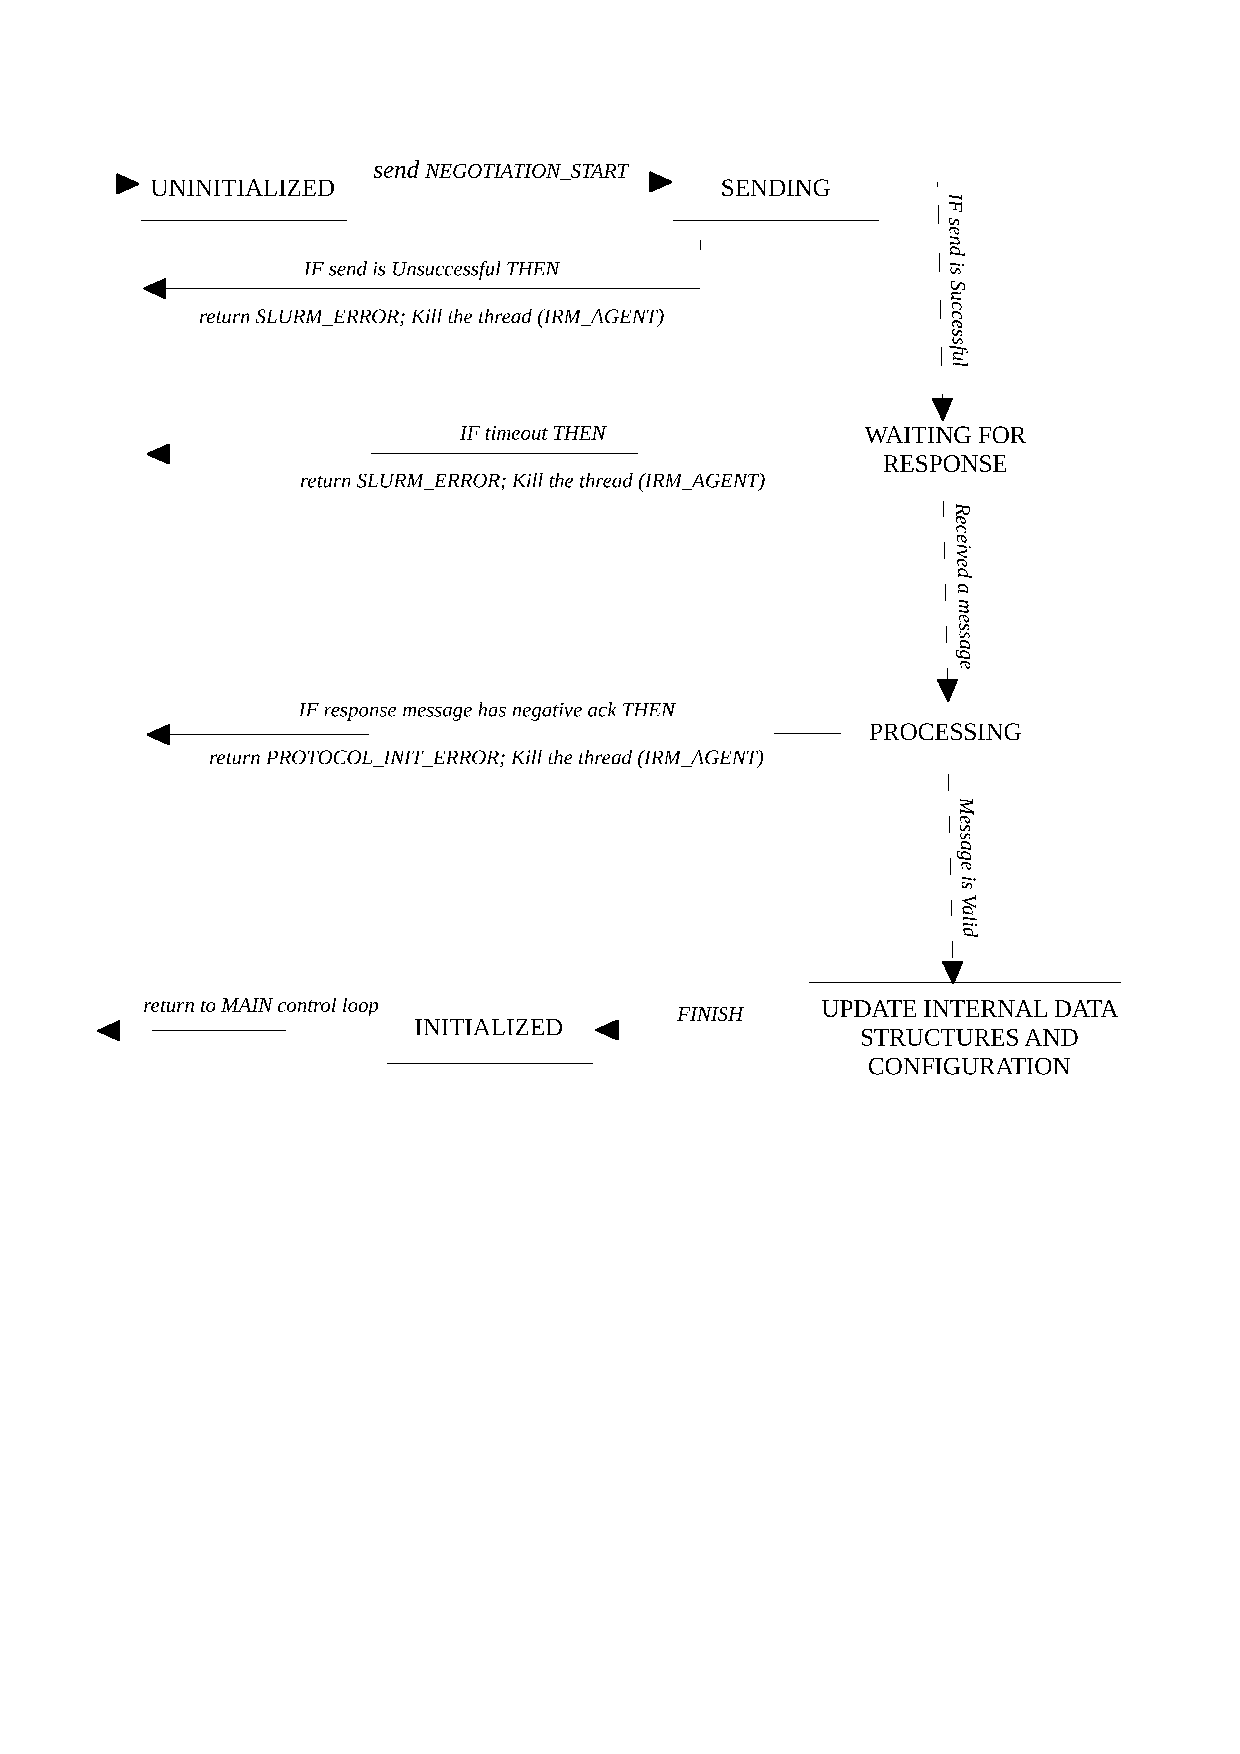
\includegraphics[width=0.9\textwidth, height=90mm]{./figures/Init.pdf}
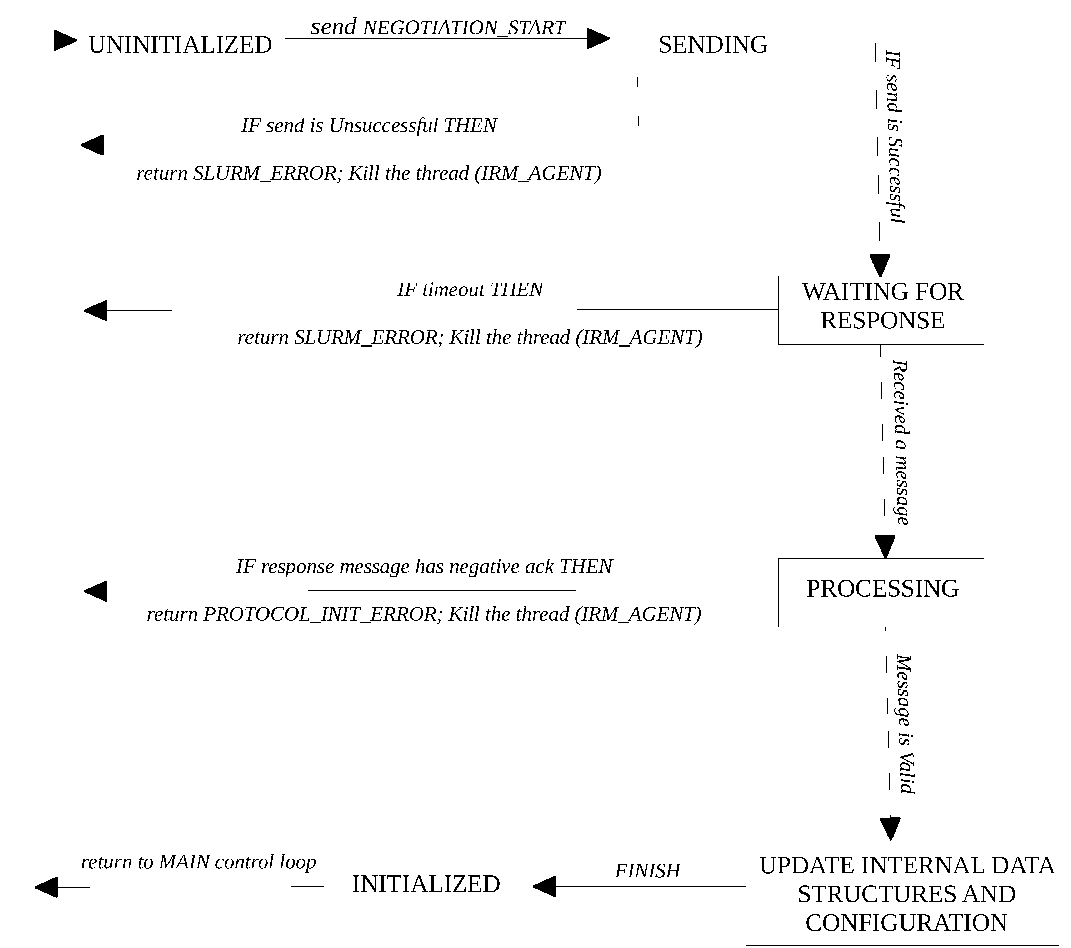
\includegraphics[width=0.9\textwidth, height=90mm]{./figures/Init.eps}
\caption{Protocol Initialization}
\label{fig:Init}
\end{figure}
\vspace{5mm}
\begin{figure}[h]
\centering
%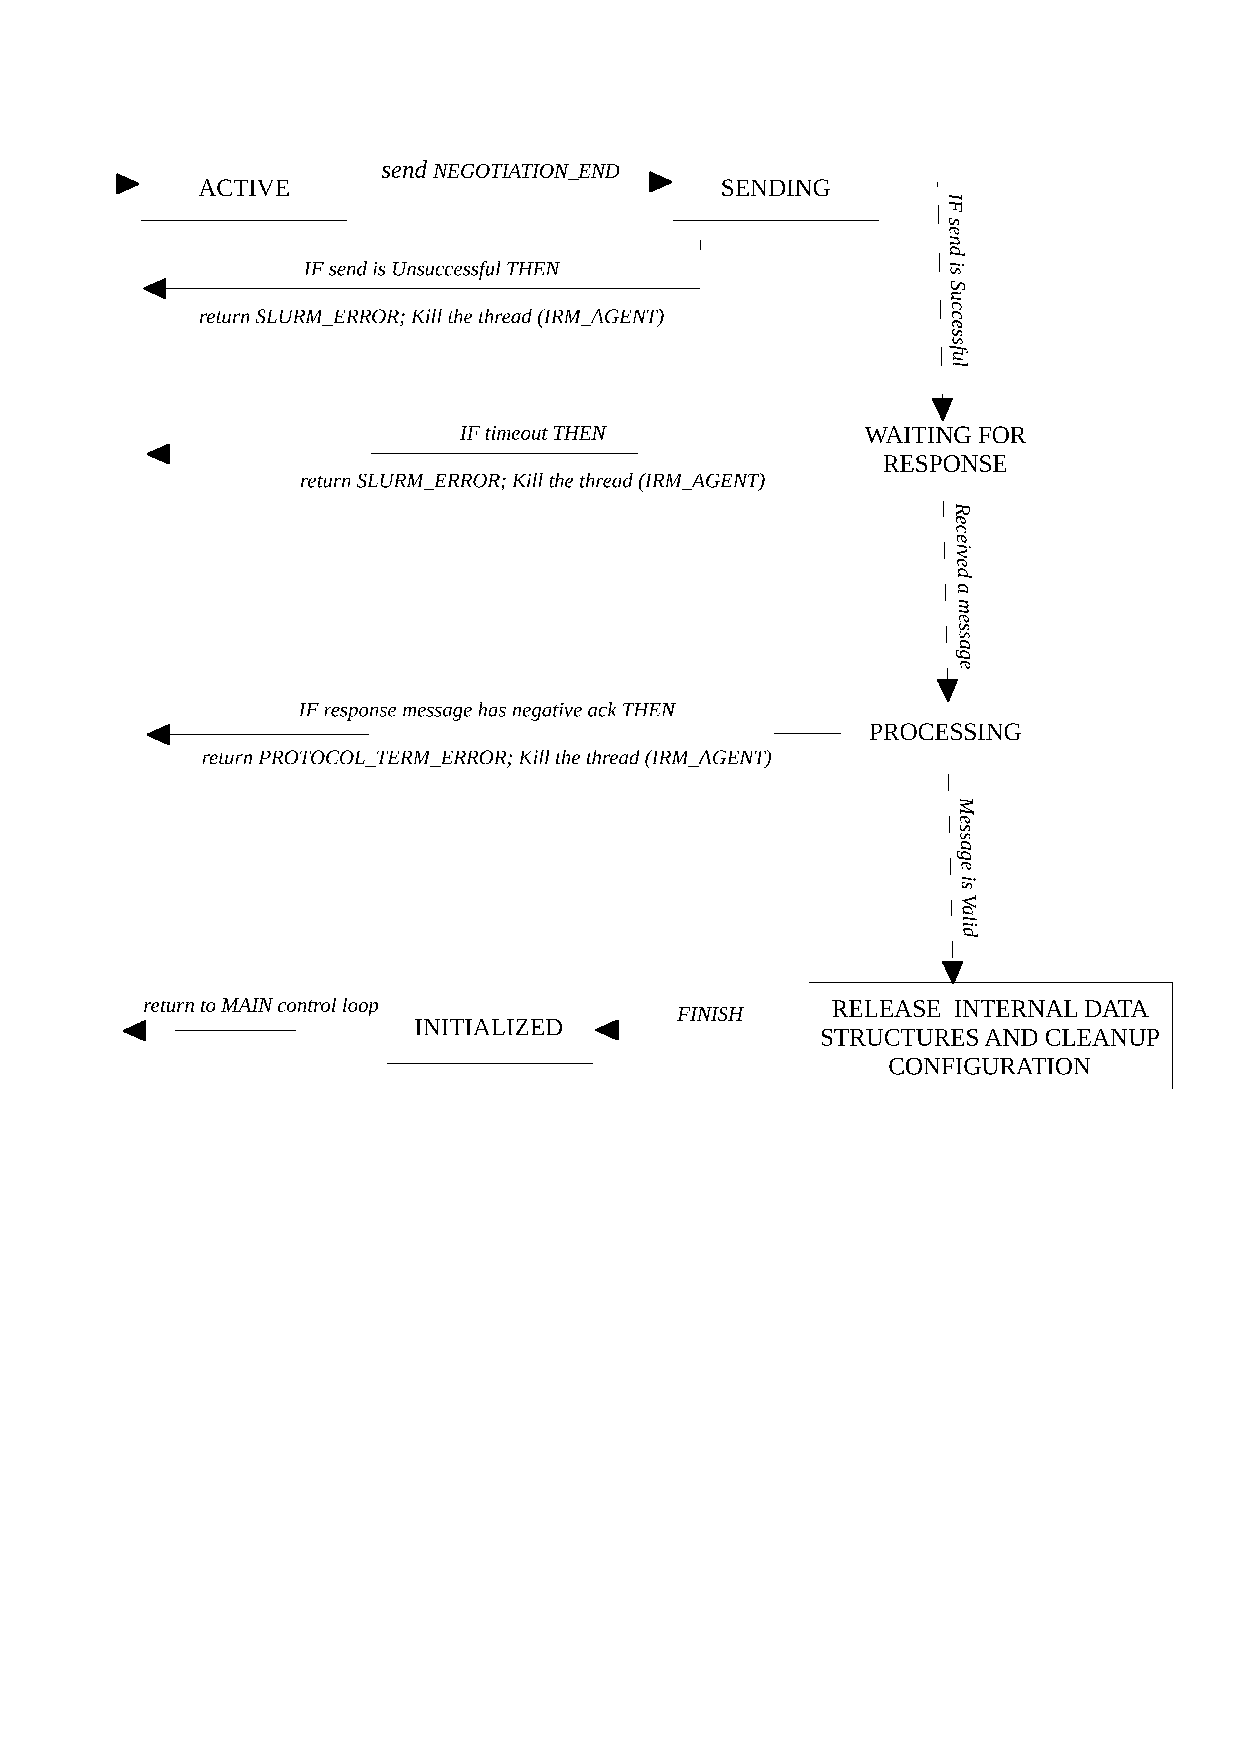
\includegraphics[width=0.9\textwidth, height=90mm]{./figures/Term.pdf}
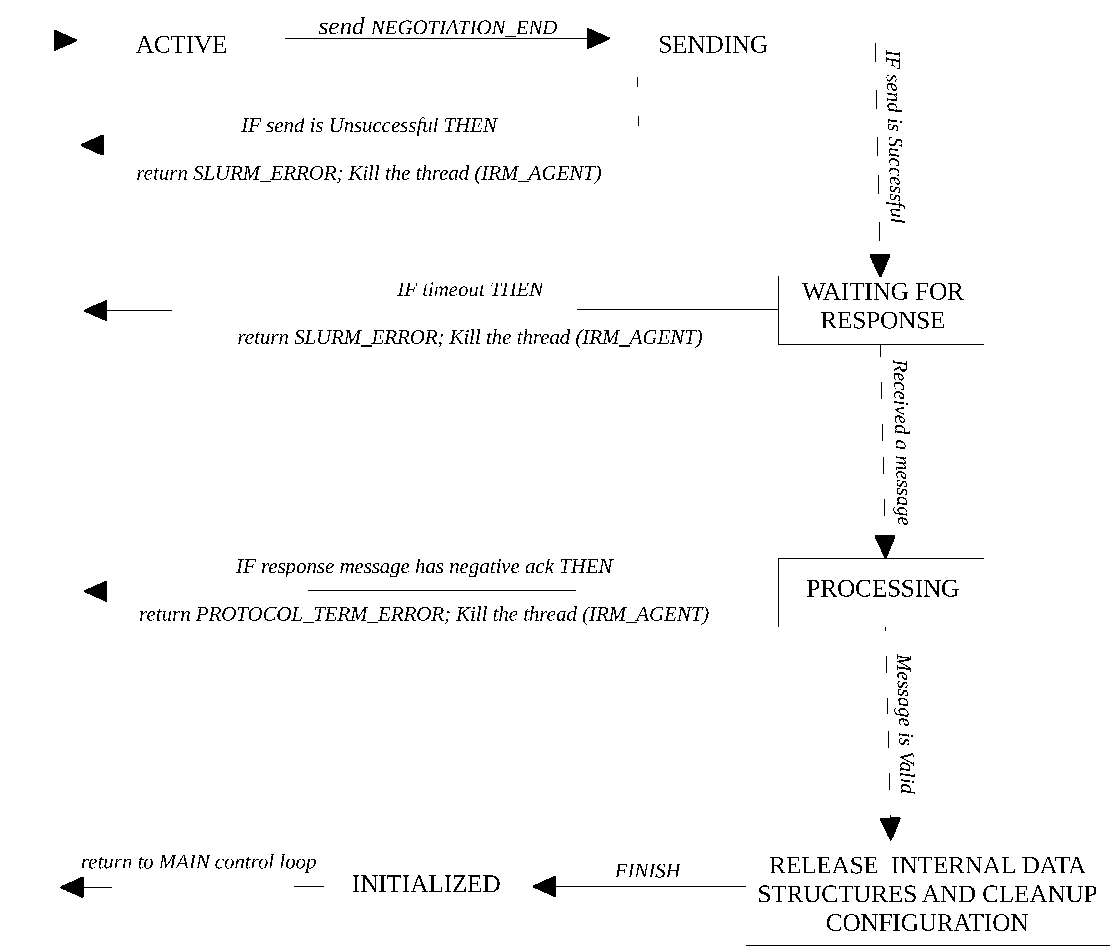
\includegraphics[width=0.9\textwidth, height=90mm]{./figures/Term.eps}
\caption{Protocol Termination}
\label{fig:Term}
\end{figure}
\clearpage
\begin{figure}[h]
\centering
%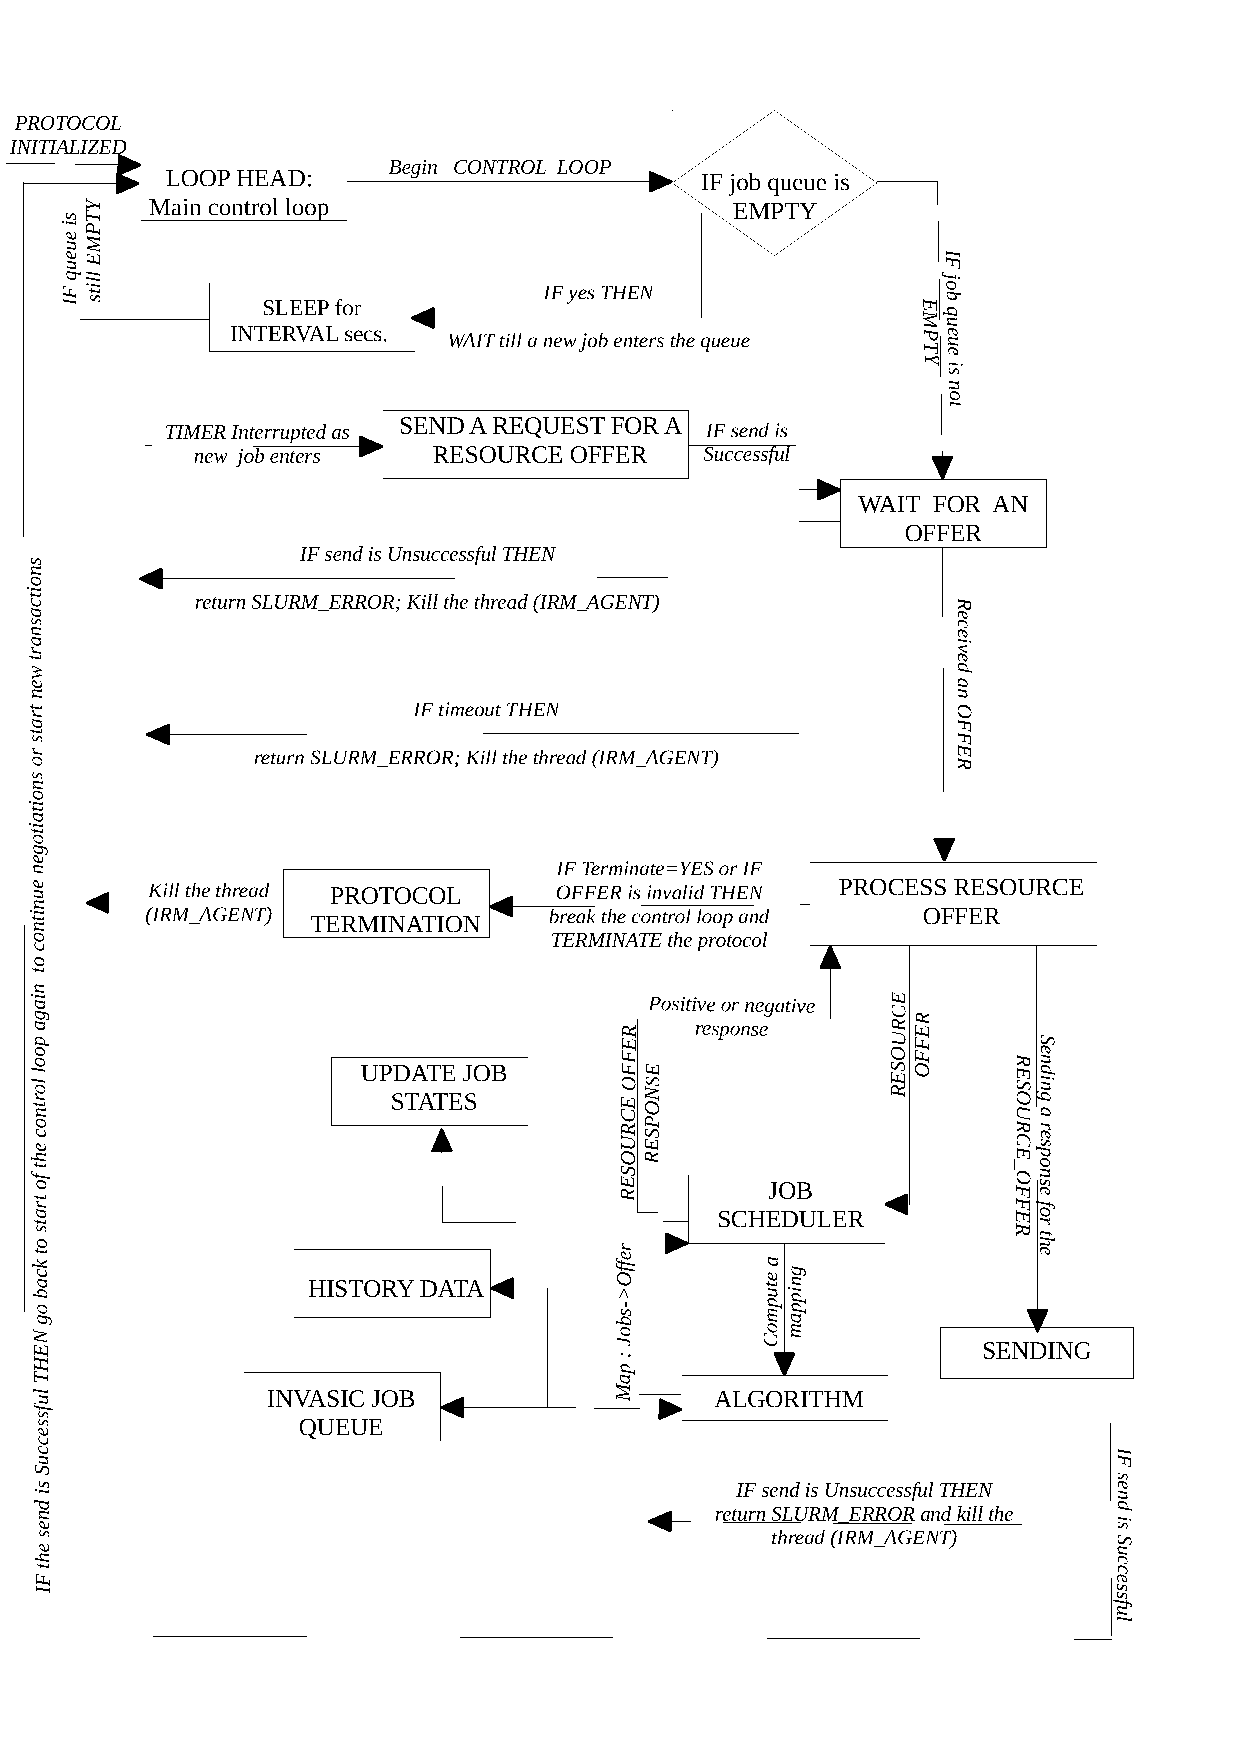
\includegraphics[width=1.0\textwidth, height=210mm]{./figures/Negotiation.pdf}
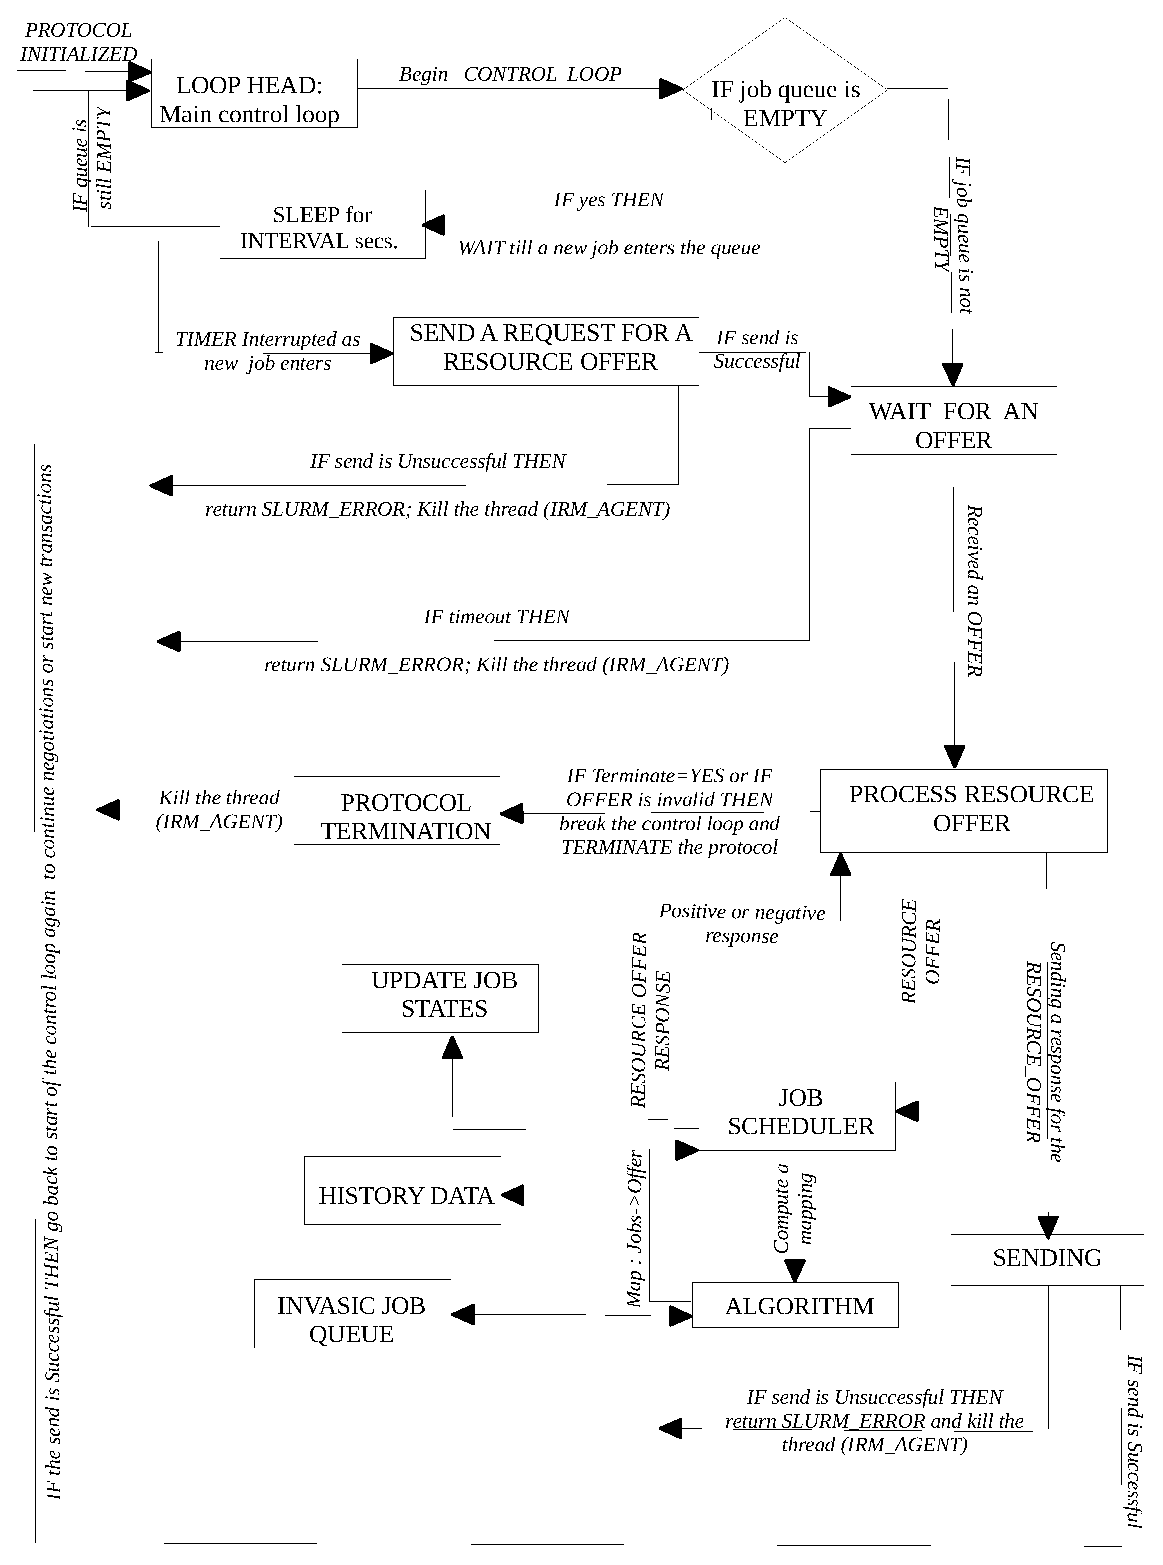
\includegraphics[width=1.0\textwidth, height=210mm]{./figures/Negotiation.eps}
\caption{Negotiation}
\label{fig:Neg}
\end{figure}
\clearpage

\section{Invasive Jobs}

\chapter{Design["How we are building". Designing the individual modules / Components, flow charts, UML diagrams, What can it do and what it cannot}\label{chapter:ischeduler}
\section{Job Mappings - Description and its generic structure}
\section{Resource Offers}
\section{Negotiation Protocol - Use state machine diagrams here}
\section{Feedback Reports}
\section{Job Scheduling Algorithms}
\subsection{Problem Formulation}
\subsection{Pseudo Code}

\chapter{Implementation}\label{chapter:implementation}
\section{Plugin}
iBSched is implemented as an extension to SLURM in the form of a scheduler plugin. A Slurm plugin is a dynamically linked code object which is loaded explicitly at run time by the Slurm libraries. A plugin provides a customized implementation of a well-defined API connected to tasks such as authentication, interconnect fabric, and task scheduling. There are several other existing scheduler plugins of SLURM such as: the default(FCFS) plugin, Backfill, wiki and wiki2(Interfaces to external schedulers) etc. A related plugin that is of importance to scheduling is the priority plugin because the job queue is first constructed and then sorted based on priorities before the scheduling algorithm runs through it. Slurm provides a basic priroity plugin and a multifactor priority plugin. The basic version provides a standard FIFO based job priority whereas the multifactor version provides priorities to job based on several factors such as age, fair-share, job size(also considers the job duration to calculate a weight factor for job size relative to time), partition, quality of service etc. The multifactor priority plugin has been refactored for this work to be better suitable for our implementation. Specifically, the multifactor priority plugin now assigns priority to jobs based on age and size(also considers the job duration to calculate a weight factor for job size relative to time). As its default behavior it also re-calculates periodically the priority of the jobs.\\ \\
%%%%%
For the current scope of the work, iRTSched has been implemented as an independent binary that talks to iBSched via the negotiation protocol. The purpose of this independent binary is to fake an actual runtime scheduler by simulating the runtime states of the system in time by employing the runtime scheduling algorithm and also negotiating with iBSched. In reality, a full-fledged runtime scheduler will be managing the resources in the invasic partition, will launch the jobs and perform dynamic resource management. In order to evaluate the negotiation-based separation of batch and runtime scheduling system, a simulation of the same involving a fake runtime scheduler would be very useful and sufficient for our objectives. 
\section{Data Structures}
This section will enumerate some of the important data structures that are a part of the implementation.\\ \\
\textbf{Job Mappings}
\begin{lstlisting}[mathescape]
enum job_hint {
        COMP_BOUND,
        MEMORY_BOUND,
        IO_BOUND,
	NONE
};

enum job_type {
        RIGID,
        MOLDABLE,
        EVOLVING,
        MALLEABLE
};

typedef struct qos_rsrc {   
        uint32_t min;
        uint32_t max;
} qos_rsrc_t;
\end{lstlisting}
%%%%%%%%
\begin{lstlisting}[mathescape]
struct forward_job_details {
        qos_rsrc_t node_count;          /* Job resource requirements */
        uint16_t contiguous;            /* set if requires contiguous nodes */
        uint16_t cpus_per_task;         /* number of processors required for
                                         * each task */
        uint8_t hint;                   /* Job characteristic: IO / Compute / Memory bound */
        uint8_t job_type;                       /* Type of job: Static or Dynamic */
        uint32_t max_cpus;              /* maximum number of cpus */
        uint32_t min_cpus;              /* minimum number of cpus */

        /* job constraints: */
        uint32_t pn_min_cpus;           /* minimum processors per node */
        uint32_t pn_min_memory;         /* minimum memory per node (MB) OR
                                         * memory per allocated
                                         * CPU | MEM\_PER\_CPU */
        uint32_t pn_min_tmp_disk;       /* minimum tempdisk per node, MB */
        uint8_t share_res;              /* set if job can share resources with
                                         * other jobs */
        uint8_t whole_node;             /* 1: --exclusive * 2: --exclusive=user */
};
\end{lstlisting}
%%%%%%%
\begin{lstlisting}[mathescape]
struct forward_job_record {
        struct forward_job_details *details;    /* job details */
        uint32_t job_id;                /* job ID */
        uint32_t magic;                 /* magic cookie for data integrity */
        char *name;                     /* name of the job */
        bitstr_t *node_bitmap;          /* bitmap of nodes allocated to job */
        uint32_t node_cnt;              /* Current node count assigned */
        uint32_t min_nodes;
        uint32_t max_nodes;
        uint32_t priority;              /* relative priority of the job,
                                         * zero == held (don't initiate) */
        time_t start_time;              /* Expected or Actual start time */
        uint32_t time_limit;            /* time_limit minutes or INFINITE,
                                         * NO_VAL implies partition max_time */
        uint32_t time_min;              /* minimum time_limit minutes or
                                         * INFINITE,
                                         * zero implies same as time_limit */
};
\end{lstlisting}
%%%%%%%
\begin{lstlisting}[mathescape]
typedef struct request_resource_offer_msg {
        uint16_t value; /* info */
        List jobs2map; /* This is the list of jobs waiting to be dispatched. And communicates the current requirements to rt scheduler which 
                          can then try to suitably construct a resource offer to satisfy the requirements as best as possible */
} request_resource_offer_msg_t;
\end{lstlisting}
%%%%%%%%
\begin{lstlisting}[mathescape]
typedef struct resource_offer_resp_msg {
        uint16_t value;         /* info */
        List map_jobs2offer;    /* Jobs mapped to the given offer. This depends on whether the batch scheduler accepted / rejected / countered
                                 the resource offer it received */
        uint32_t error_code;    /* error code on failure */
        char   * error_msg;     /* error message on failure */
} resource_offer_resp_msg_t;
\end{lstlisting}
%%%%%%%
\textbf{Resource Offers}
\begin{lstlisting}[mathescape]
typedef struct job_resv {
        time_t end_time;        /* end time of reservation              */
        uint8_t full_nodes;        /* when reservation uses full nodes or not */
        uint32_t job_id;        /* job ID */
        bitstr_t *node_bitmap;  /* bitmap of reserved nodes             */
        uint32_t node_cnt;      /* count of nodes required              */
        time_t start_time;      /* start time of reservation            */
} job_resv_t;


typedef struct resource_offer_msg {
        uint16_t value;      /* info */
        uint8_t negotiation; /* if negotiation is ongoing then this value is 1 else it becomes 0 to indicate ischeduler that previous negotiat
                                ion is over */
        List resource_offer;   /* List of node space records */
        List resv_jobs;        /* List of jobs with actual reservations. Can also include jobs with virtual reservations that are those with
                                  future start / service times */
        uint32_t error_code;    /* error code on failure */
        char   * error_msg;     /* error message on failure */
} resource_offer_msg_t;
\end{lstlisting}
%%%%%%%%%%
\textbf{Feedback Reports}
\begin{lstlisting}[mathescape]
typedef struct job_status {
        uint32_t job_id;
        time_t run_time;
        time_t end_time;
        uint32_t node_cnt;
        bitstr_t *node_bitmap;
        uint32_t job_state;
} job_status_t;

typedef struct status_report_msg {
        List status_reports;
} status_report_msg_t;
\end{lstlisting}
%%%%%%%%%%%
\textbf{Running Job Record}
\begin{lstlisting}[mathescape]
struct run_job_record {
        uint32_t job_id;
        bitstr_t *node_bitmap;
        time_t start_time;
        uint32_t priority;
        uint32_t time_limit;
        uint8_t hint;
        uint8_t job_type;
        time_t end_time;
        time_t orig_end_time;
        uint32_t job_state;
        uint32_t orig_node_cnt;
        uint32_t node_cnt;
        uint32_t last_node_cnts[2];
        bitstr_t *next_node_bitmap;
        uint32_t next_node_cnt;
        uint32_t depend_job_id;
        uint32_t depend_job_prio;
        uint32_t save_depend_job_id;
        uint32_t save_depend_job_prio;
        uint32_t min_nodes;
        uint32_t max_nodes;
        uint8_t adapt;  /* 0 - No change, 1 - Expand, 2 - Shrink */
        uint8_t transformed;
        time_t exp_end_time;
        time_t last_resize_time;
        uint32_t adapt_interval;
};
\end{lstlisting}
%%%%%%%
\textbf{Node Space Map}
\begin{lstlisting}[mathescape]
typedef struct node_space_map {
        time_t begin_time;
        time_t end_time;
        bitstr_t *avail_bitmap;
        int next;       /* next record, by time, zero termination */
} node_space_map_t;
\end{lstlisting}
%%%%%%%%
\section{Important APIs}
For batch scheduler\\
\begin{lstlisting}[mathescape]
extern List schedule_invasic_jobs(resource_offer_msg_t *, List, uint16_t *, uint32_t *);

extern uint32_t adjustQoS_node_count(struct job_record *);

extern void resetQoS_node_counts();

extern int _decision_logic(List, int, uint32_t);

extern void *irm_agent(void *);

extern int receive_resource_offer(slurm_fd_t, slurm_msg_t *);

extern int process_resource_offer(resource_offer_msg_t *, uint16_t *, int *, List *, List);

extern int send_resource_offer_resp(slurm_msg_t *, char *, List);

extern int request_resource_offer(slurm_fd_t, List);

extern int _request_resource_offer(slurm_fd_t);  /* Wrapper for request_resource_offer to construct the list of job requirements to be sent */
\end{lstlisting}
%%%%%%%%%%%%%
For runtime scheduler\\
\begin{lstlisting}[mathescape]
extern int slurm_submit_resource_offer(slurm_fd_t, resource_offer_msg_t *, resource_offer_resp_msg_t **);

extern int wait_req_rsrc_offer (slurm_fd_t, request_resource_offer_msg_t **);

extern int process_rsrc_offer_resp(resource_offer_resp_msg_t *, int, resource_offer_msg_t **);

extern int compute_feedback(status_report_msg_t *);

extern int create_resource_offer(int, List, uint16_t, resource_offer_msg_t **);

extern bitstr_t * _try_transf(bool);

extern int _commit_state(bool);

extern bitstr_t * _restore_state(void);

extern int _update_job_states(void);

extern time_t next_job_endtime(void);

extern bool _get_delta(uint32_t *, time_t, time_t);

extern void _initialize_state(void);

extern int _decision_logic(resource_offer_msg_t *, List, int, bool);
\end{lstlisting}
%%%%%%%%%%%%%
\section{State Machine Diagrams}
\subsection{iBSched}
\begin{figure}[!t]
\centering
\includegraphics[width=1.0\textwidth, height=210mm]{./figures/iBSched.pdf}
%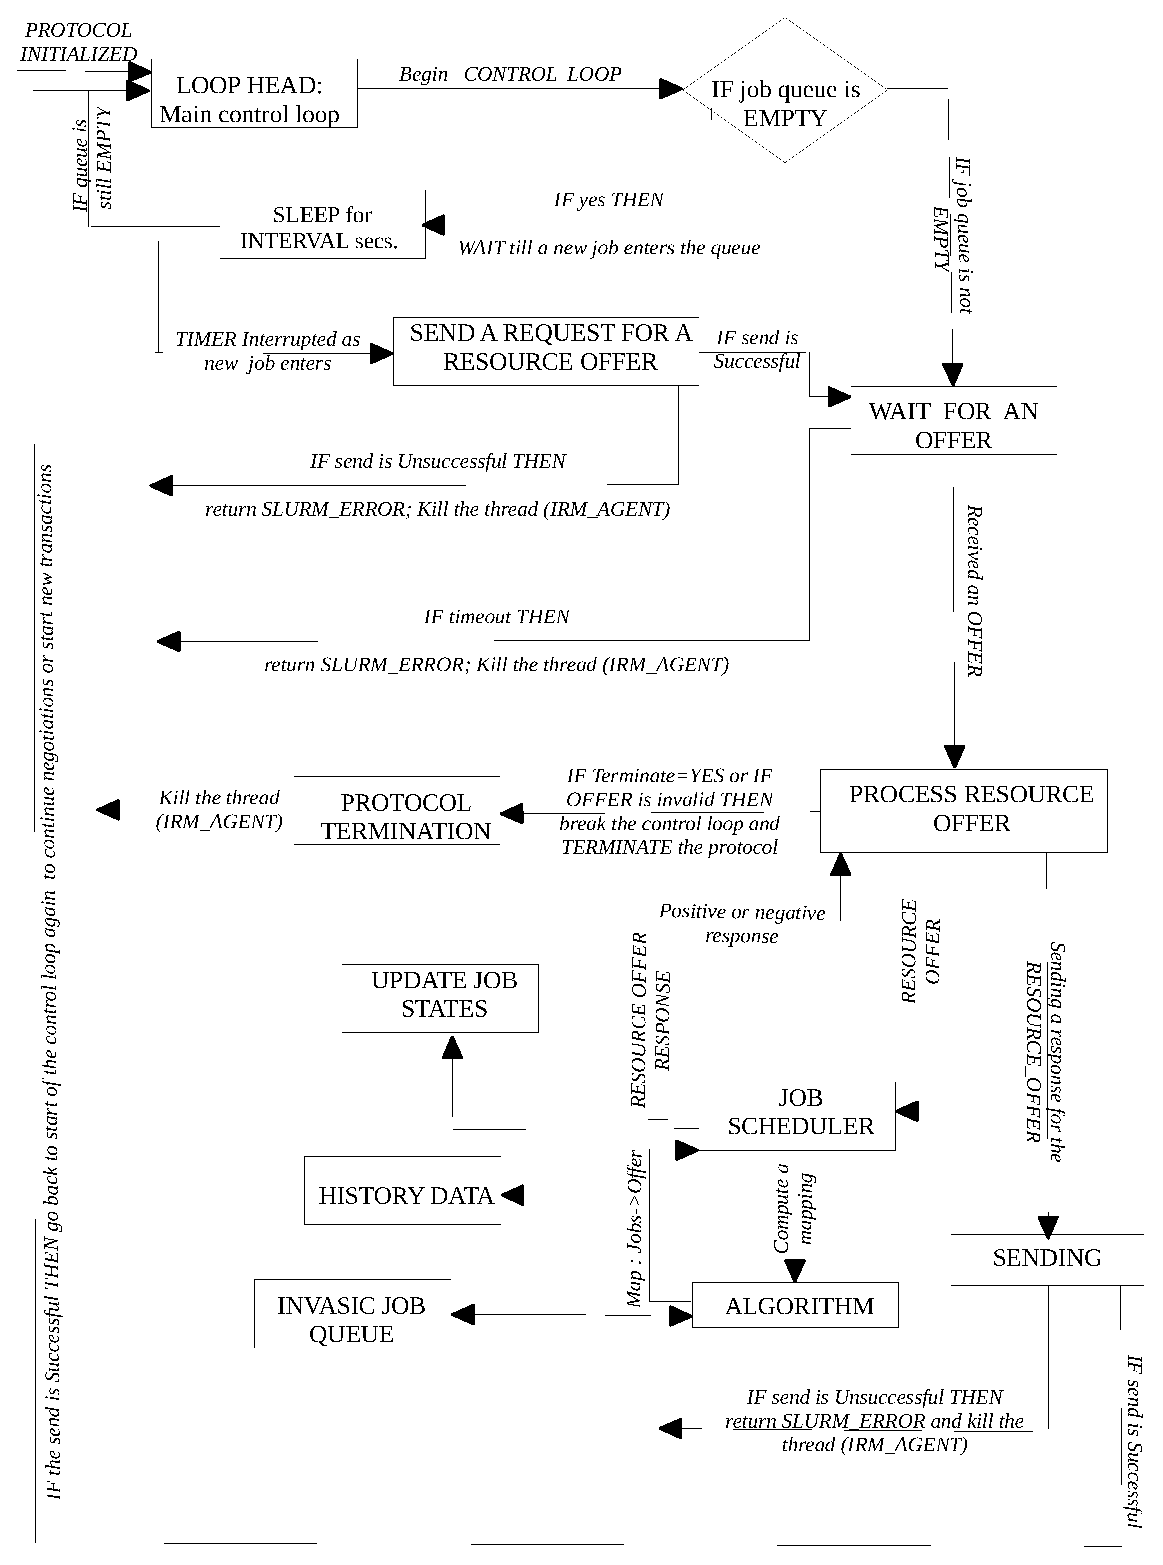
\includegraphics[width=1.0\textwidth, height=180mm]{./figures/Negotiation.eps}
\caption{iBSched}
\label{fig:Neg}
\end{figure}
\subsection{iRTSched}
\begin{figure}[!htbp]
\centering
%\includegraphics[width=1.0\textwidth, height=180mm]{./figures/iBSched.eps}
%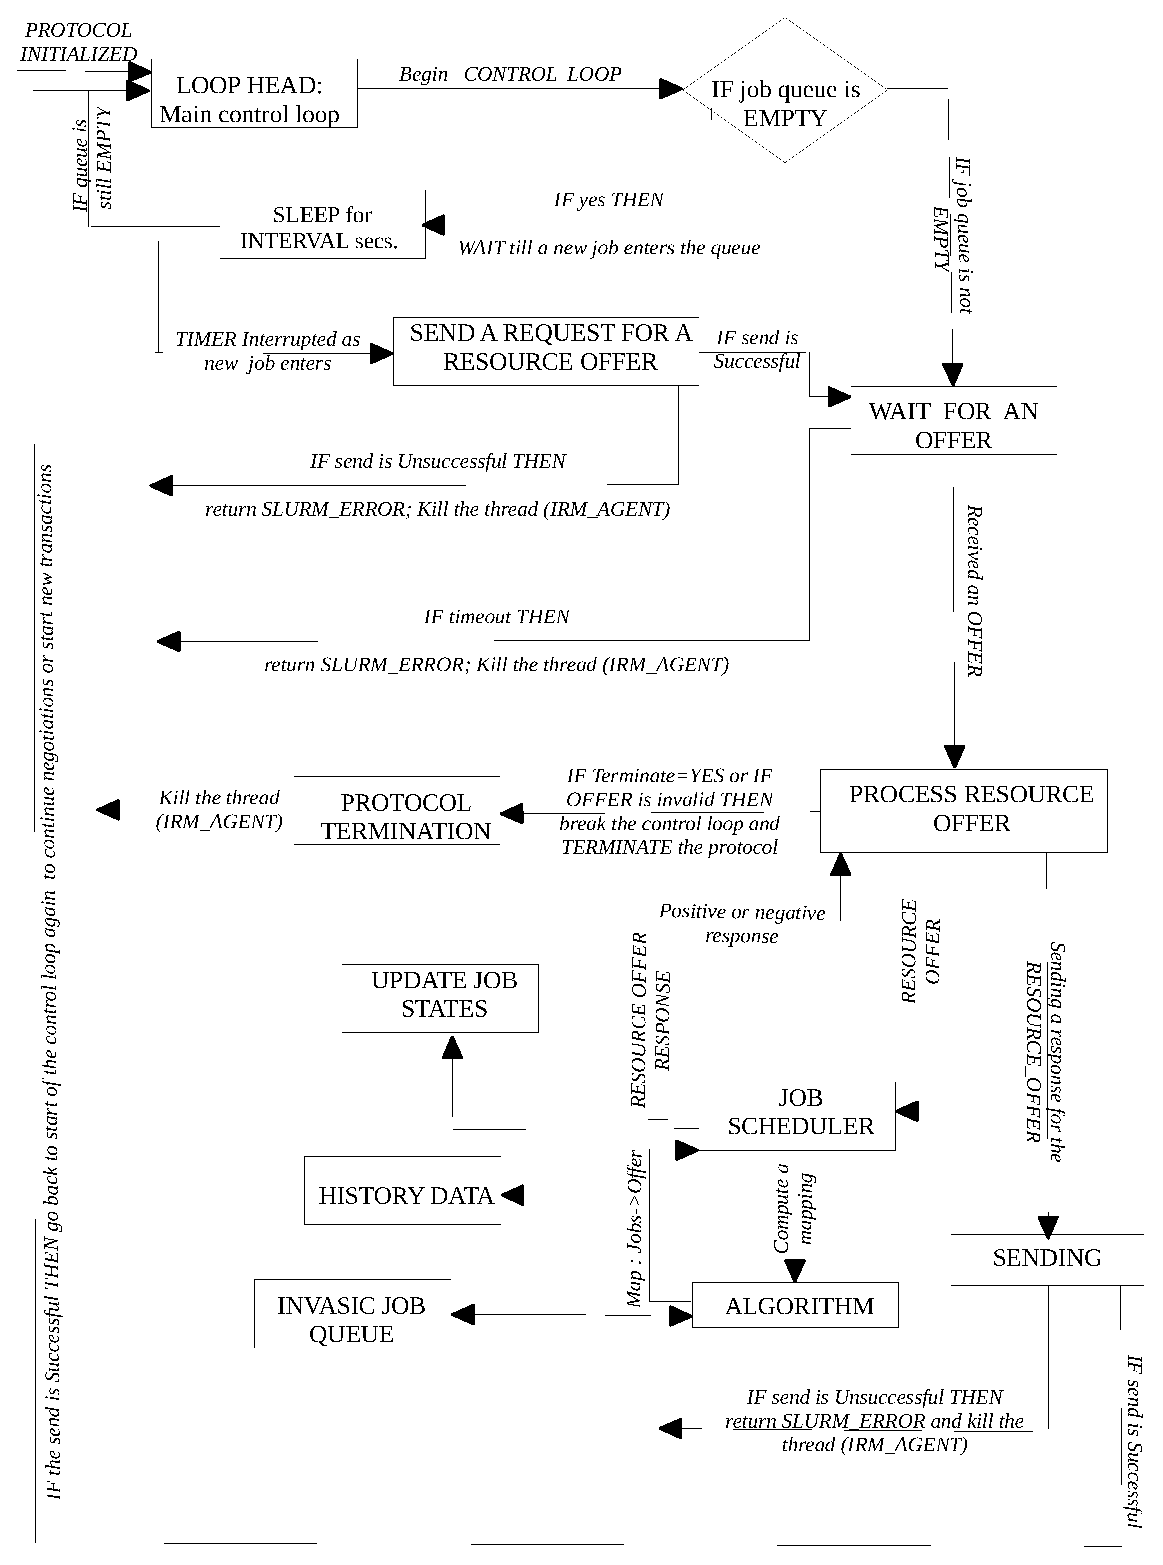
\includegraphics[width=1.0\textwidth, height=180mm]{./figures/Negotiation.eps}
\caption{iRTSched}
\label{fig:Neg}
\end{figure}

\chapter{Evaluation}\label{chapter:evaluation}
May be a page illustrating a scenario of negotiation with 2d node space map diagrams will be good.
\section{Method of Evaluation}
\subsection{Emulation of Workload}
\subsection{Real Invasic Applications}
\section{Setup}
\section{Experiments and Results}
\section{Performance and Graphs}

\chapter{Conclusion and Future Work}\label{chapter:conclusion and future}
<TBA>
\section{Future Work}
<Dummy citations of papers to test if bibliography section is working fine>
\cite{felix}
\cite{laxmikant}
\cite{nikolas}
\cite{rudolph}
\cite{isaias}
\cite{andreas}
\cite{georgiou}
\cite{travis}
\cite{gladys}
\cite{klein}
\cite{pavan}
\cite{jette}
\cite{abhishek}
\cite{david}
\cite{joseph}
\cite{hungershofer}
\cite{yangjie}
\cite{zhou}
\cite{lucero}
\cite{desai}
\cite{yang}
\cite{daniel}
\cite{dror}
\cite{ahuva}
\cite{dinesh}
\cite{slurm}
\cite{tsafrir}
\cite{streit}
\cite{achim}
\cite{achim1}
\cite{streit1}
\cite{achim2}
\cite{striet2}
\cite{deshmeh}
\cite{tiachao}
\cite{oliver}
\cite{alain}
\cite{viktor}
\cite{rizos}
\cite{viktor1}
\cite{javier}
\cite{kwang}
\cite{kurowski}
\cite{ariel}
\cite{roland}
\cite{cirne}
\cite{desai}
\cite{michal}
\cite{sudha}
\cite{srividya}
\cite{song}
\cite{sabin}
\cite{dalibor}
\cite{osman}
\cite{rajesh}
\cite{calvin}
\cite{sudarshan}
\cite{ribbens}
\cite{vadhiyar}
\cite{gonzalo}
\cite{martin}
\cite{gonzalo1}
\cite{maria}
\cite{srinidhi}
\cite{jamjoom}
\cite{zhiling}
\cite{siham}
\cite{deshmeh2010adept}
\cite{wcirne}
\cite{wcirne1}
\cite{daniel1}
\cite{da2015exascale}
\cite{dongxu}
\cite{buisson}
\cite{striet2}
\cite{schulz}
\cite{wong}
\cite{teich}

% TODO: add more chapters here

\appendix{}

 % TODO: remove if glossary not needed
%\glsaddall{} % add all defined terms to glossary, even if not referenced in text
%\printglossaries{}

\microtypesetup{protrusion=false}
\microtypesetup{protrusion=true}
\printbibliography{}

\end{document}
